\documentclass[compress]{beamer}
\usepackage{ifthen,verbatim}

\newcommand{\isnote}{}
\xdefinecolor{lightyellow}{rgb}{1.,1.,0.25}
\xdefinecolor{darkblue}{rgb}{0.1,0.1,0.7}

%% Uncomment this to get annotations
%% \def\notes{\addtocounter{page}{-1}
%%            \renewcommand{\isnote}{*}
%% 	   \beamertemplateshadingbackground{lightyellow}{white}
%%            \begin{frame}
%%            \frametitle{Notes for the previous page (page \insertpagenumber)}
%%            \itemize}
%% \def\endnotes{\enditemize
%% 	      \end{frame}
%%               \beamertemplateshadingbackground{white}{white}
%%               \renewcommand{\isnote}{}}

%% Uncomment this to not get annotations
\def\notes{\comment}
\def\endnotes{\endcomment}

\setbeamertemplate{navigation symbols}{}
\setbeamertemplate{headline}{\mbox{ } \hfill
\begin{minipage}{5.5 cm}
\vspace{-0.75 cm} \small
\end{minipage} \hfill
\begin{minipage}{4.5 cm}
\vspace{-0.75 cm} \small
\begin{flushright}
\ifthenelse{\equal{\insertpagenumber}{1}}{}{Jim Pivarski \hspace{0.2 cm} \insertpagenumber\isnote/\pageref{numpages}}
\end{flushright}
\end{minipage}\mbox{\hspace{0.2 cm}}\includegraphics[height=1 cm]{../cmslogo} \hspace{0.1 cm} \includegraphics[height=1 cm]{../tamulogo} \hspace{0.01 cm} \vspace{-1.05 cm}}

\begin{document}
\begin{frame}
\vfill
\begin{center}
\textcolor{darkblue}{\Large Summary of Current Global-Distortion Knowledge \\ \vspace{0.2 cm} and Tools for Resolving them in General}

\vfill
\begin{columns}
\column{0.3\linewidth}
\begin{center}
\large
\textcolor{darkblue}{Jim Pivarski}
\end{center}
\end{columns}

\begin{columns}
\column{0.3\linewidth}
\begin{center}
\scriptsize
{\it Texas A\&M University}
\end{center}
\end{columns}

\vfill
19 March, 2010

\end{center}
\end{frame}

%% \begin{notes}
%% \item This is the annotated version of my talk.
%% \item If you want the version that I am presenting, download the one
%% labeled ``slides'' on Indico (or just ignore these yellow pages).
%% \item The annotated version is provided for extra detail and a written
%% record of comments that I intend to make orally.
%% \item Yellow notes refer to the content on the {\it previous} page.
%% \item All other slides are identical for the two versions.
%% \end{notes}

\small

\begin{frame}
\frametitle{Summary}
\begin{itemize}
\item There is evidence that a persistent effect in muon residuals is
  due to a global distortion of the tracker
\begin{itemize}
\item it is probably a tracker-$\chi^2$-invariant weak mode, resolved
  by the external information--- the muon chamber hits
\end{itemize}

\item Strongest indication is that a true tracker weak mode, generated
  intentionally with Millepede, reproduces/cancels some of the
  features of the bias

\item The effect is not fully understood, but is too important to ignore
\begin{itemize}
\item shape of the apparent bias:

\vspace{0.2 cm}
{\hspace{-1.5 cm}\begin{minipage}{1.2\linewidth}\scriptsize
$\displaystyle \Delta \kappa(p_T, \phi, \theta) - \Delta \kappa(p_T \to 0, \phi, \theta) = (0.0005\mbox{ GeV}^{-1}) \sin(\phi - 0.7) \exp\left(-\frac{(100\mbox{ GeV})^2}{{2 \, p_T}^2}\right)$
\end{minipage}\mbox{\hspace{-3 cm}}}

\vspace{0.2 cm}
\item implies {\it either} 2.5\% modulation of $Z$ mass in $\phi$ {\it
  or} complete washing-out of $Z'$ mass, or a little of both
\end{itemize}

\item This ``unpleasant discovery'' could be turned into a technique
  for correcting the bias and even providing definite uncertainty
  estimates on curvature bias: systematic errors for physics analyses

\end{itemize}
\end{frame}

\begin{frame}
\frametitle{Diagnostic method}
\begin{columns}
\column{0.5\linewidth}
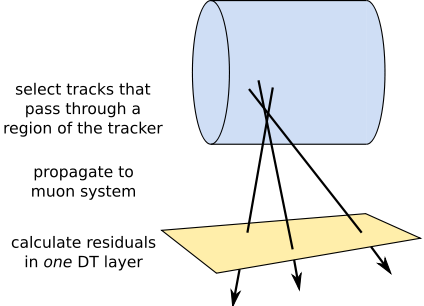
\includegraphics[width=\linewidth]{method.png}

\column{0.5\linewidth}
\begin{itemize}
\item Tracker-only track fit
\item Propagate to only one muon layer (single rigid-body alignable)
\item Dependence of residuals ($\Delta x$) on tracker-track curvature
  ($q/p_T$) cannot be attributed to muon misalignment
\end{itemize}
\end{columns}
\begin{center}
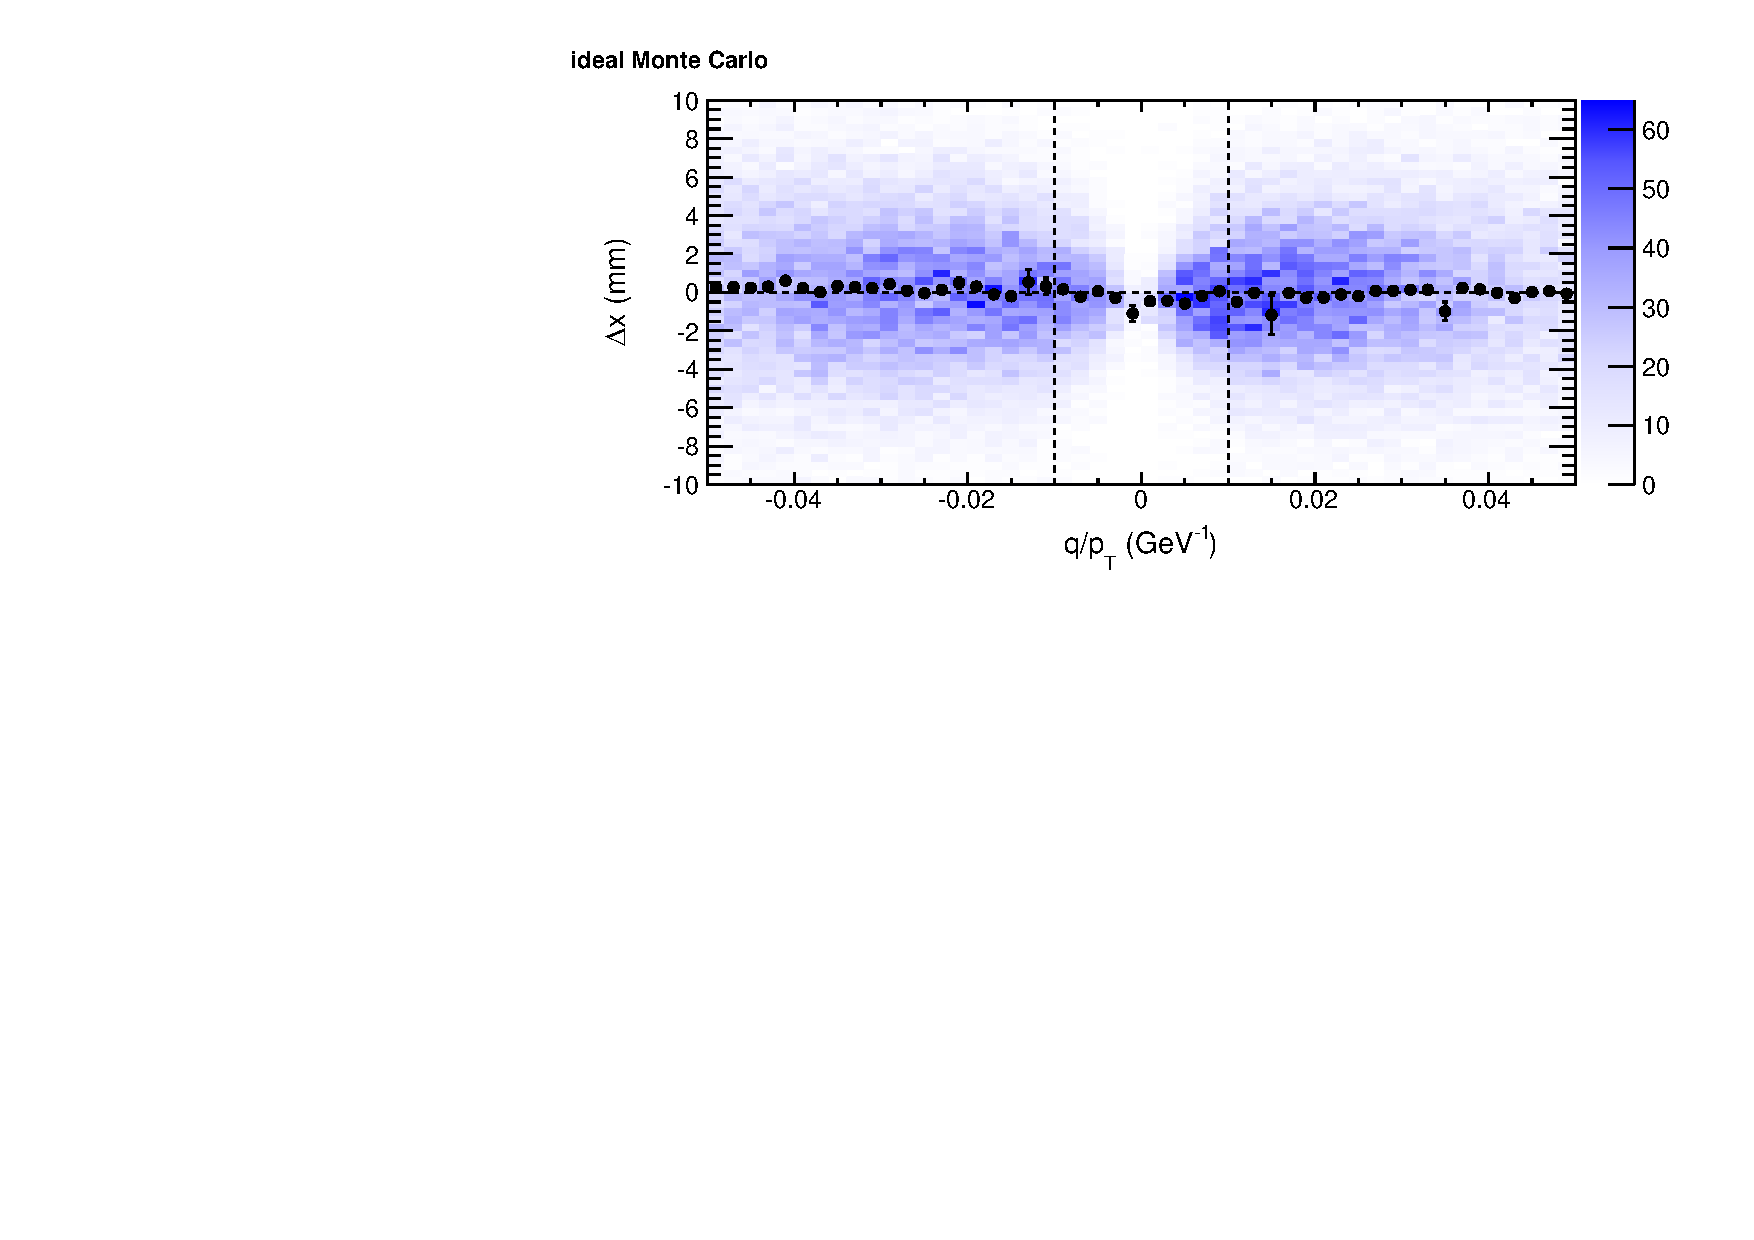
\includegraphics[width=0.6\linewidth]{residuals_ideal.pdf}
\vspace{-1 cm}
\end{center}
\end{frame}

\begin{frame}
\frametitle{The $\Delta x$ vs $q/p_T$ plot}

\begin{columns}
\column{0.35\linewidth}
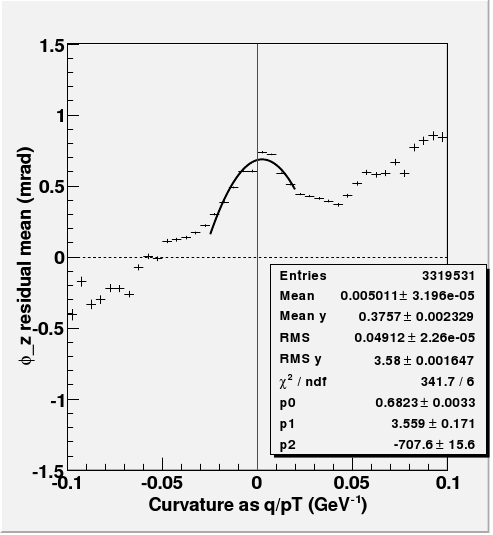
\includegraphics[width=\linewidth]{old_Deltax_vs_qoverpT.png}

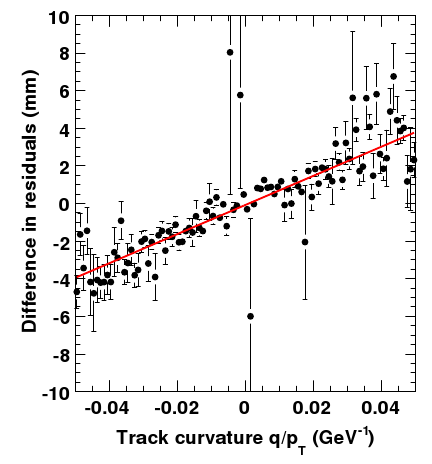
\includegraphics[width=\linewidth]{old_Deltax1-Deltax2_vs_qoverpT.png}
\column{0.65\linewidth}
\begin{itemize}
\item Originally made to distinguish alignment errors from magnetic field map errors
\item Top: first plot, Dec~2008, rough because all chambers combined
  (not yet aligned), shows the high-momentum feature
\item Bottom-left: a more focused plot, single sector, $\Delta x_1 - \Delta
  x_2$ for two stations, shows antisymmetric magnetic field effect but
  no high-momentum feature
\item Feature only present in residuals on tracks from
  the tracker, in both CRAFTs

\vspace{0.1 cm}
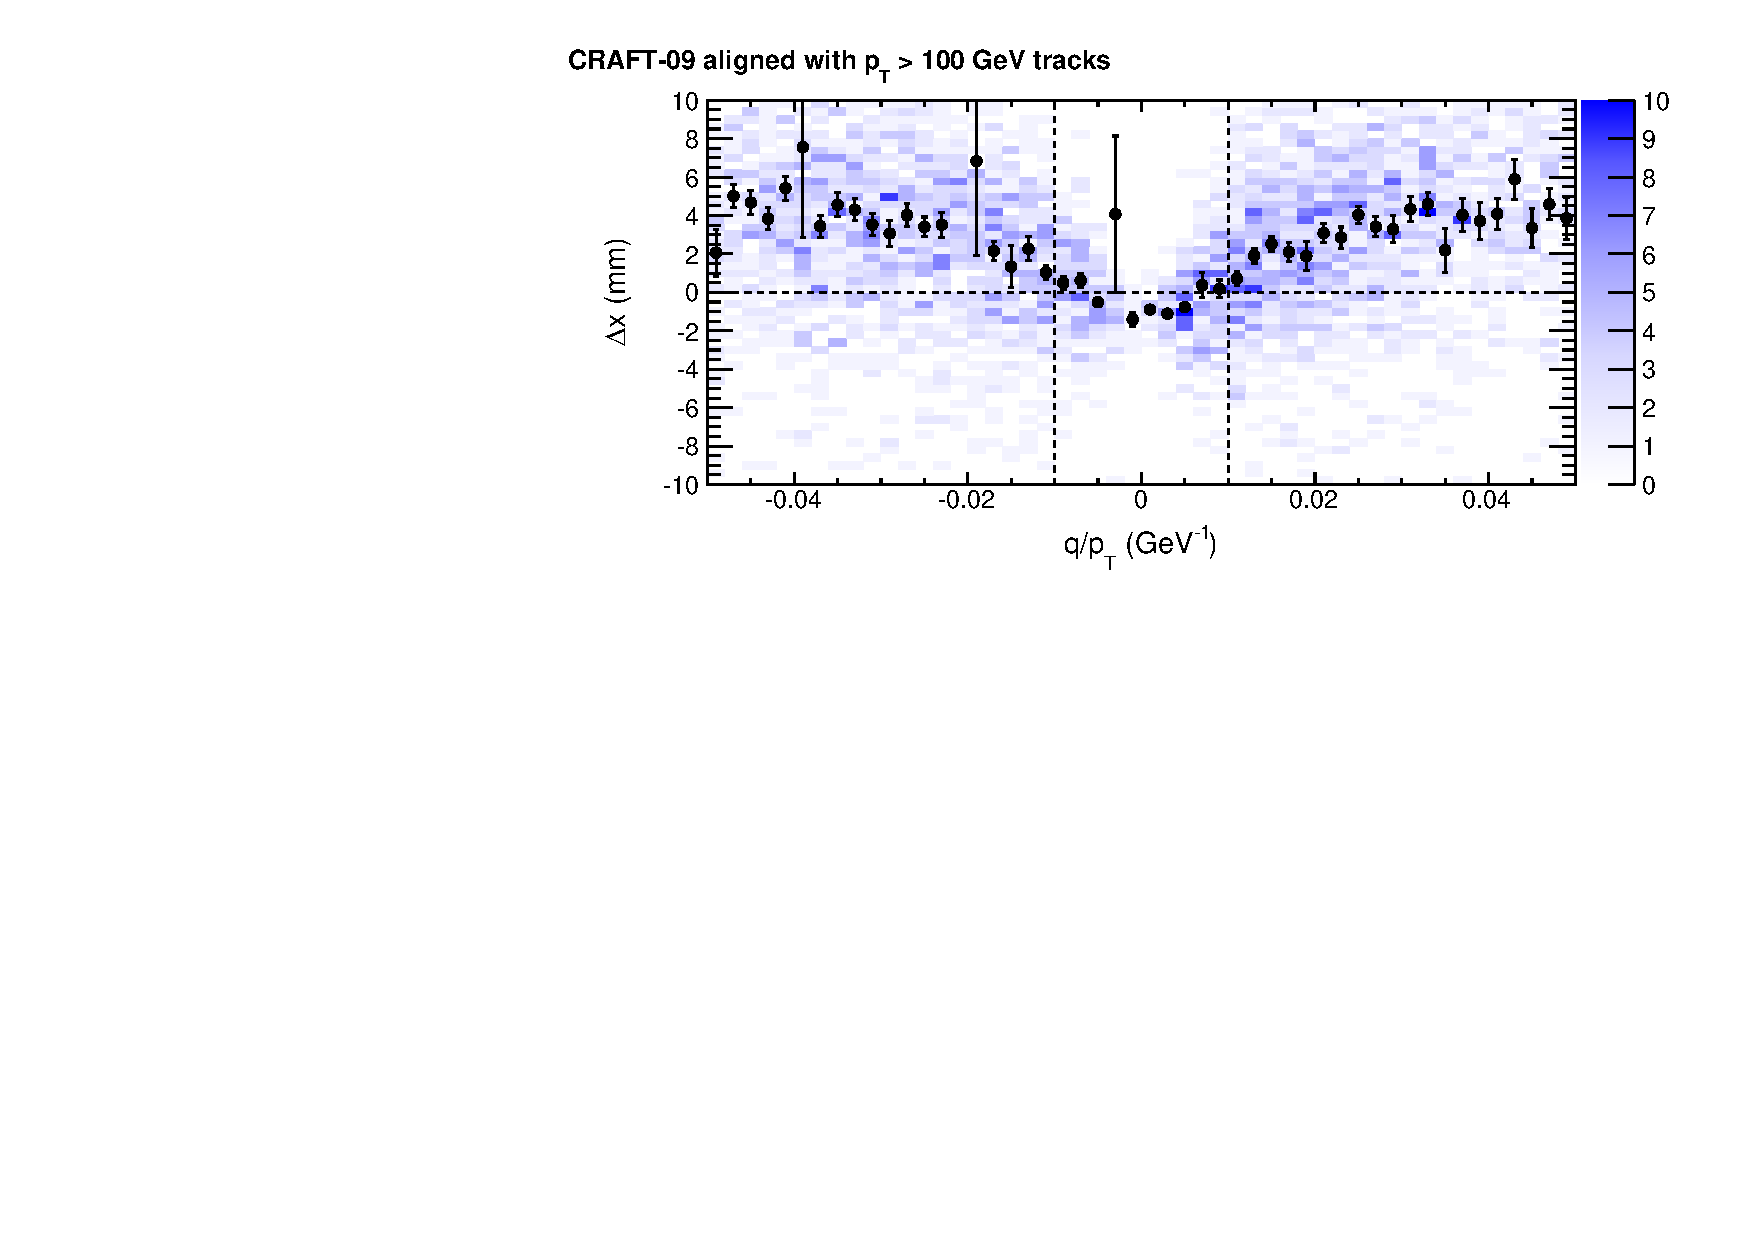
\includegraphics[width=\linewidth]{residuals_real.pdf}
\end{itemize}
\end{columns}
\end{frame}

\begin{frame}
\frametitle{Interpretation of this plot}

\begin{columns}
\column{0.5\linewidth}
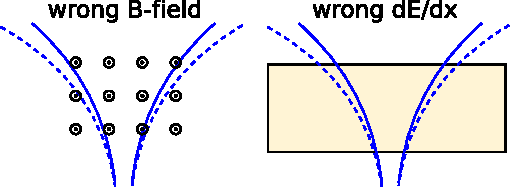
\includegraphics[width=\linewidth]{things_that_are_antisymmetric.pdf}

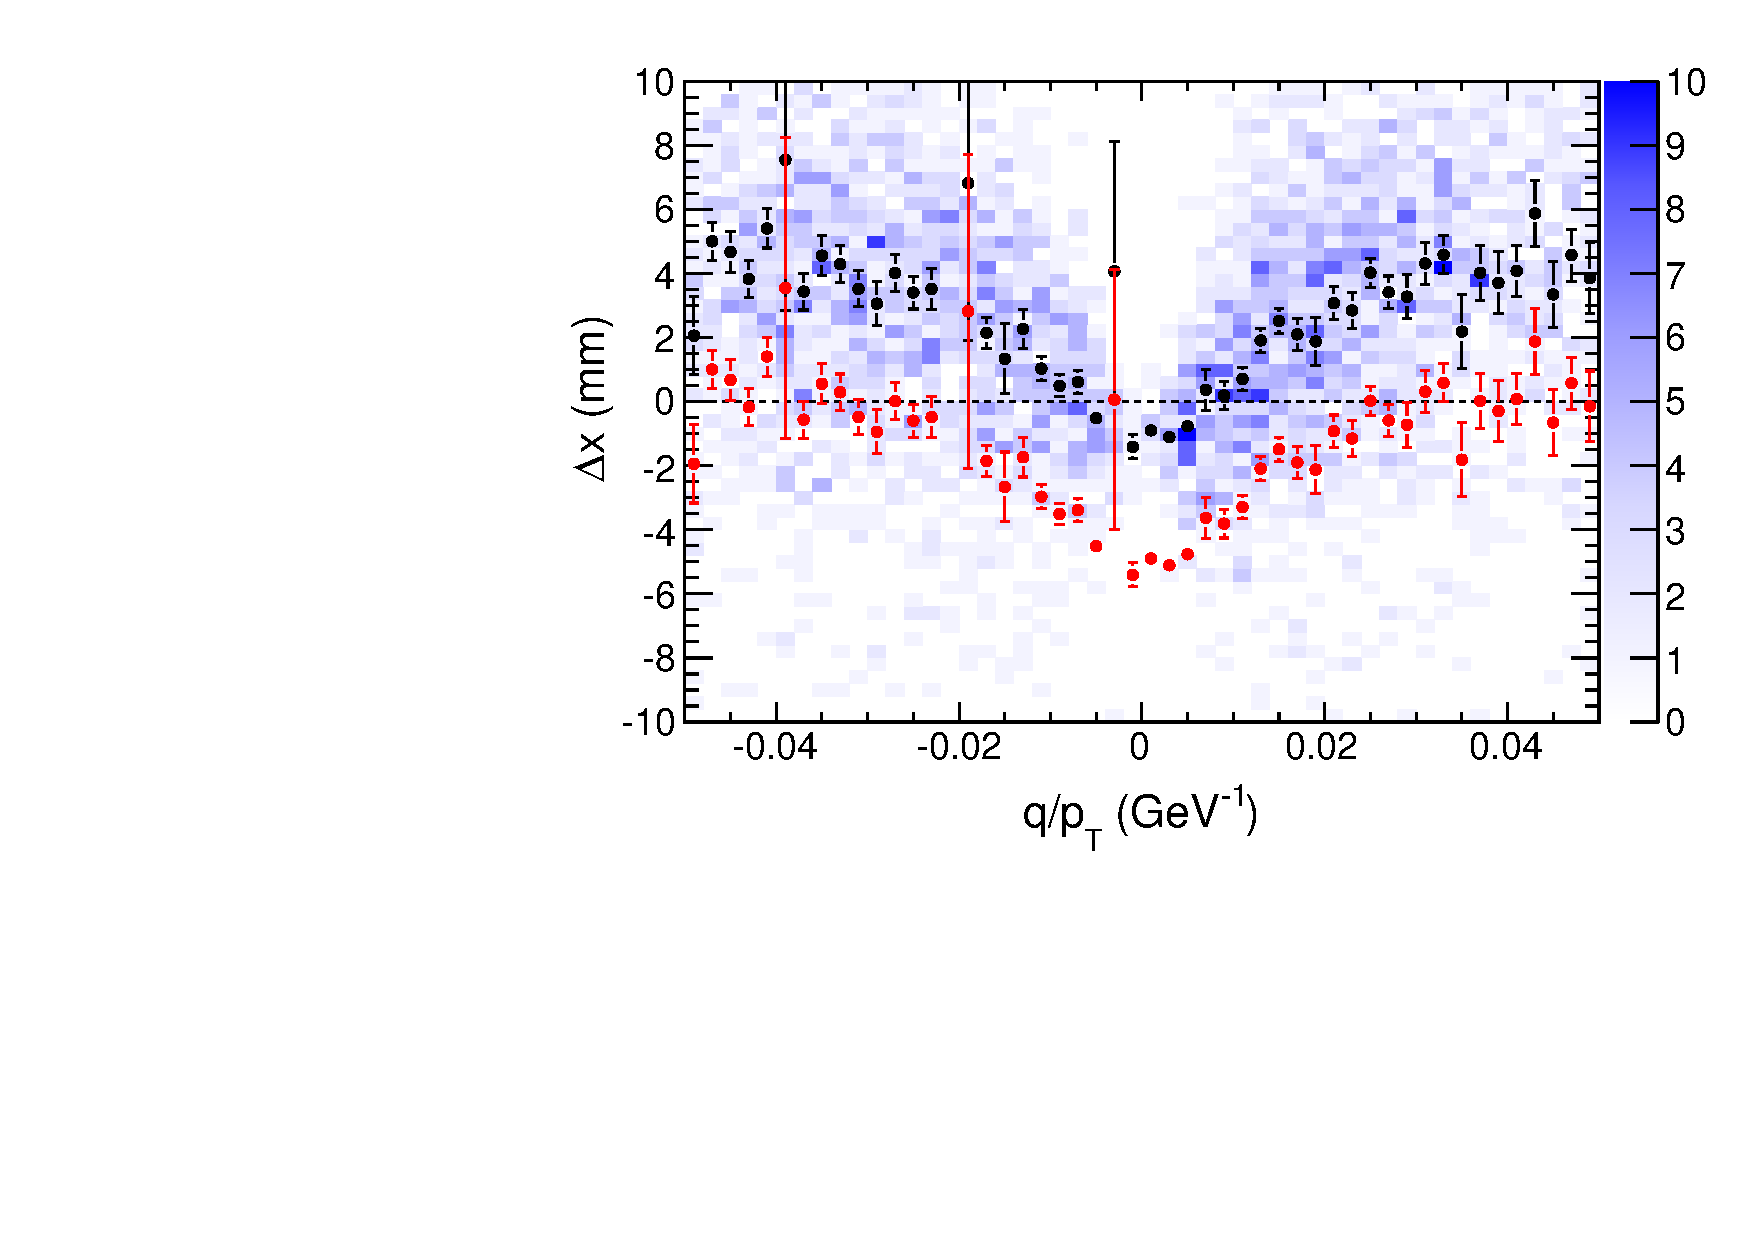
\includegraphics[width=\linewidth]{residuals_real_both.pdf}
\column{0.5\linewidth}
\begin{itemize}
\item Both magnetic field and material budget errors lead to antisymmetric effects on $\Delta x$
\begin{itemize}
\item high-momentum feature effect is therefore neither
\end{itemize}
\item When it is made with a single muon layer, layer misalignment (in
  $r\phi$) corresponds to vertical translation
\begin{itemize}
\item ignore vertical offsets
\end{itemize}
\end{itemize}
\end{columns}

\begin{itemize}
\item Transform $\displaystyle \Delta(q/p_T) = \frac{\epsilon}{x(q/p_T)
  - x(q/p_T + \epsilon)} \Delta x$, numerical \\ \vspace{0.2 cm} derivative calculated by
  running propagator twice (purely mathematical); $\Delta(q/p_T)$ vs $q/p_T$ quantifies tracker only
\end{itemize}
\end{frame}

\begin{frame}
\frametitle{What we can constrain}

\hfill 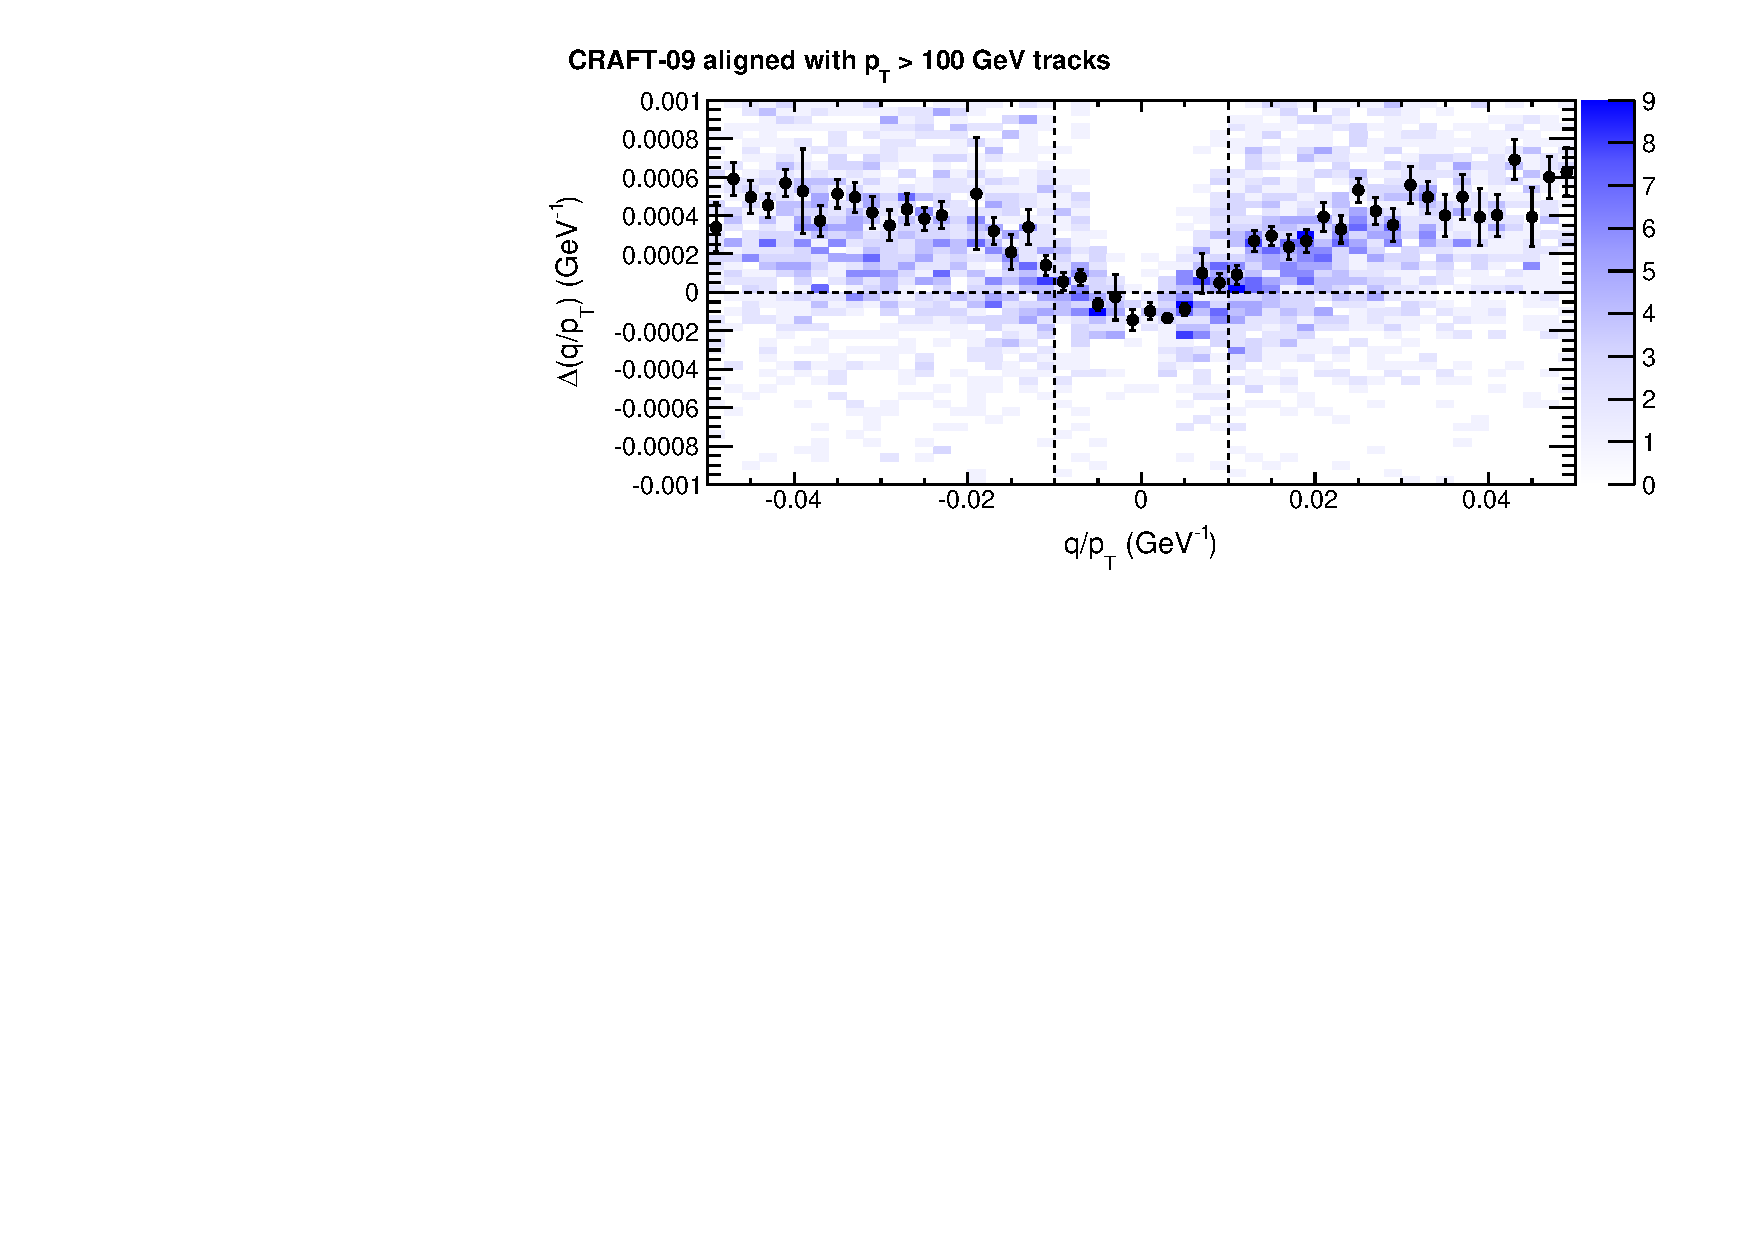
\includegraphics[width=0.5\linewidth]{curvature_real.pdf}

\vspace{-2.3 cm}
\begin{itemize}
\item $\frac{\partial x}{\partial (q/p_T)}$ is nearly 
  constant \\ vs $q/p_T$ (within a $\phi$ region), \\ so $\Delta(q/p_T)$ has
  the same \\ behavior as $\Delta x$
\begin{itemize}
\item needs to be studied as a function of $\phi$!
\end{itemize}

\item Therefore, vertical offsets in $\Delta(q/p_T)$ vs $q/p_T$ should
  be ignored, because they are equivalent to muon alignment

\item We constrain only curvature bias differences:
\begin{center}
$\Delta \kappa(\kappa, \phi, \theta) - \Delta \kappa(\kappa \to \infty, \phi, \theta)$
\end{center}
in 12 $\phi$ bins (sectors) and 5 $\cot\theta$ bins (wheels), $\kappa = q/p_T$

\item Observed form is

{\hspace{-1 cm}\begin{minipage}{1.15\linewidth}
$\displaystyle \Delta \kappa(\kappa, \phi, \theta) - \Delta \kappa(\infty, \phi, \theta) = (0.0005\mbox{ GeV}^{-1}) \sin(\phi - 0.7) \exp\left(-\frac{(100\mbox{ GeV})^2}{{2 \, p_T}^2}\right)$
\end{minipage}\mbox{\hspace{-3 cm}}}

\end{itemize}
\end{frame}

\begin{frame}
\frametitle{What led to the empirical form}

\begin{columns}
\column{0.6\linewidth}
\only<1>{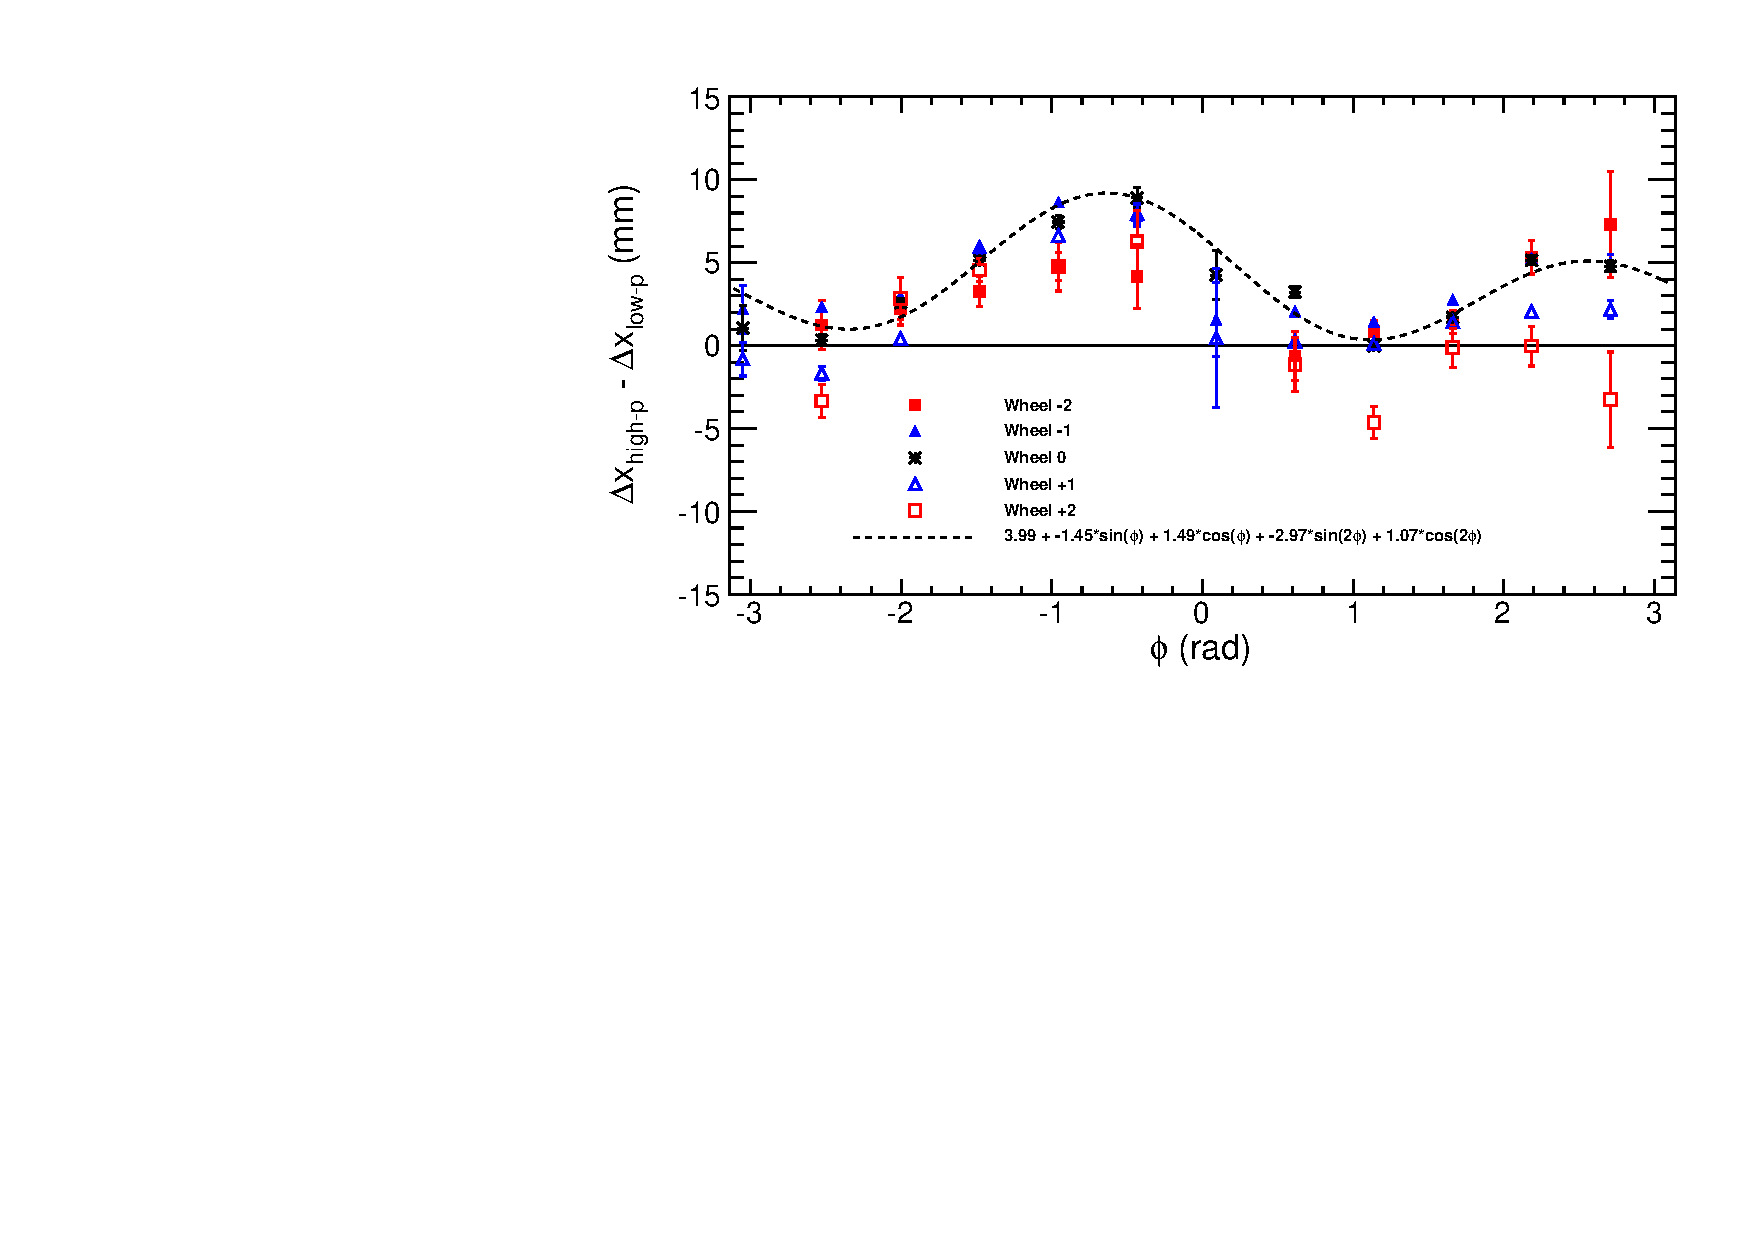
\includegraphics[width=\linewidth]{deltax_vs_phi.pdf}}
\only<2>{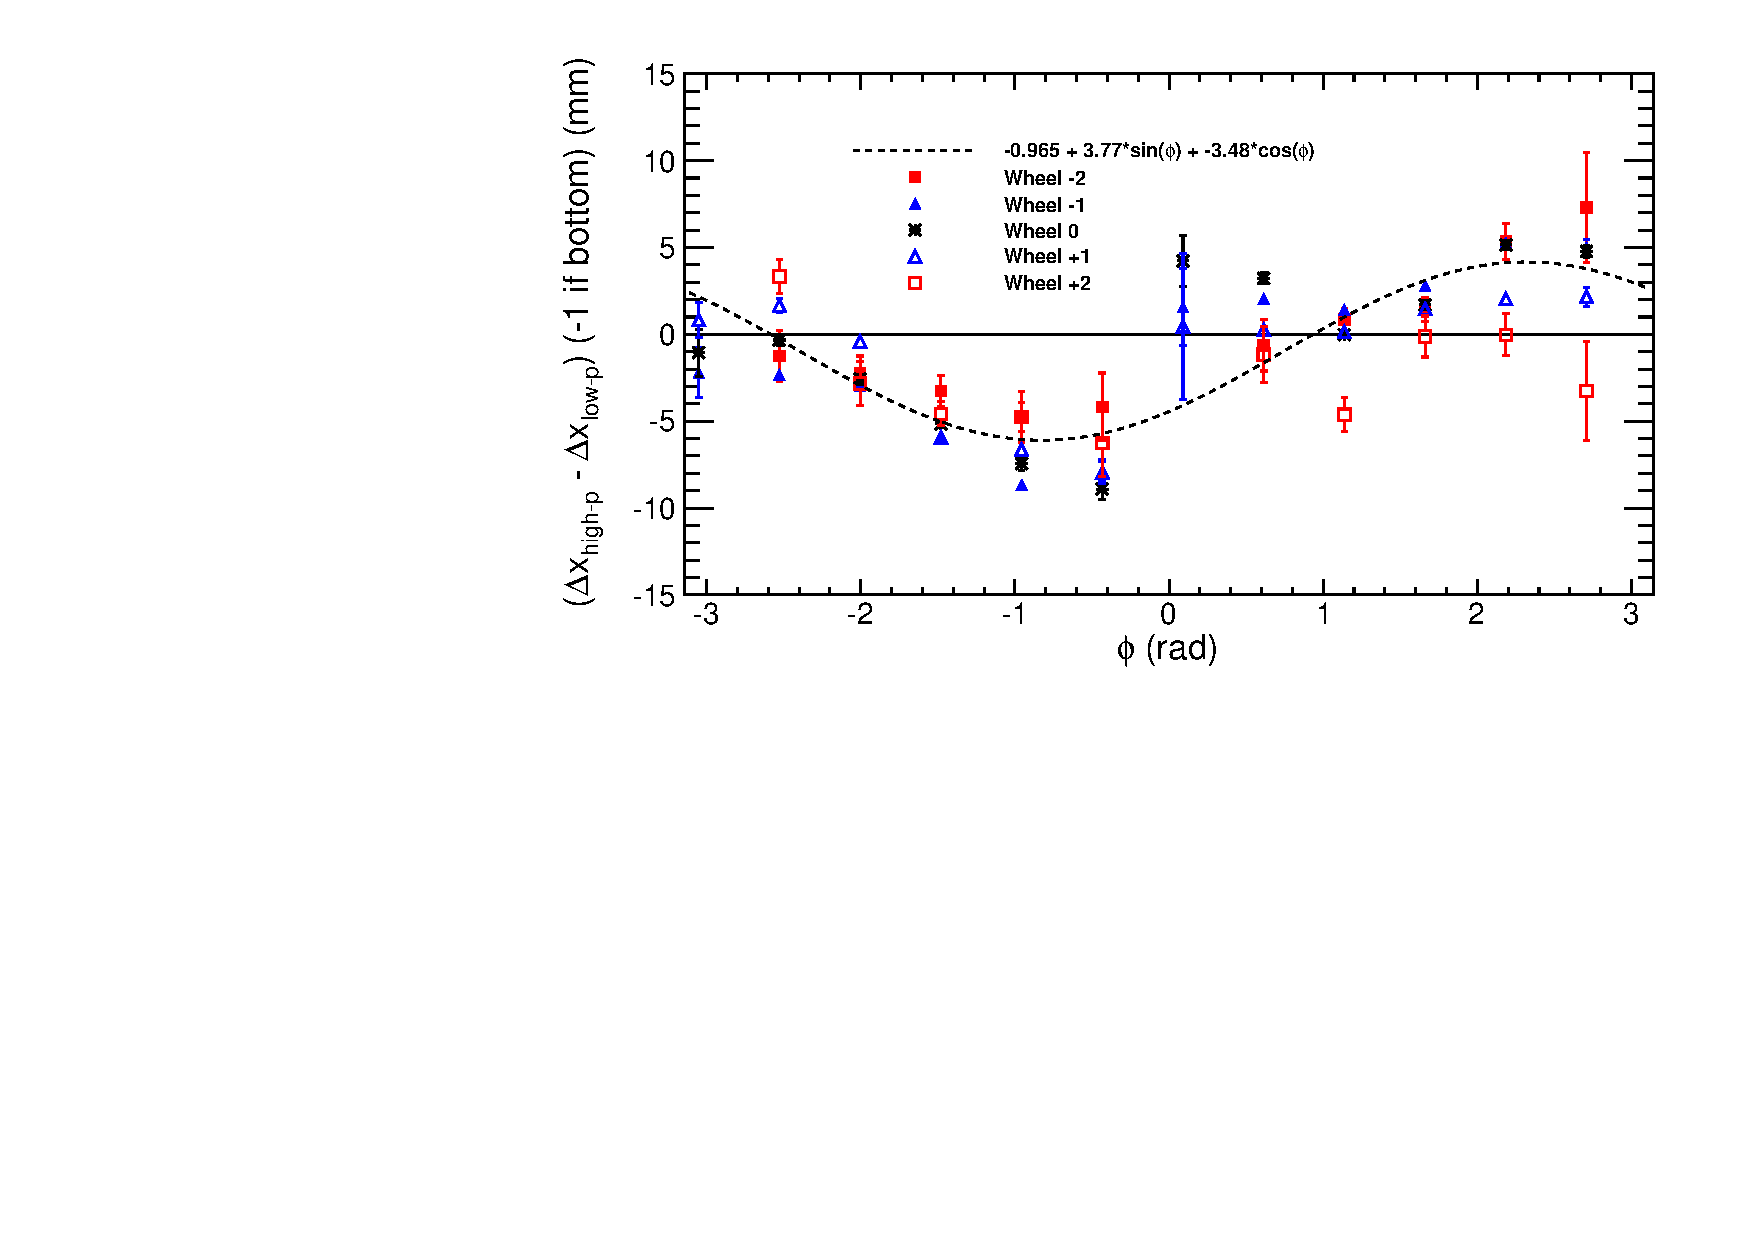
\includegraphics[width=\linewidth]{deltax_vs_phi_flipbottom.pdf}}

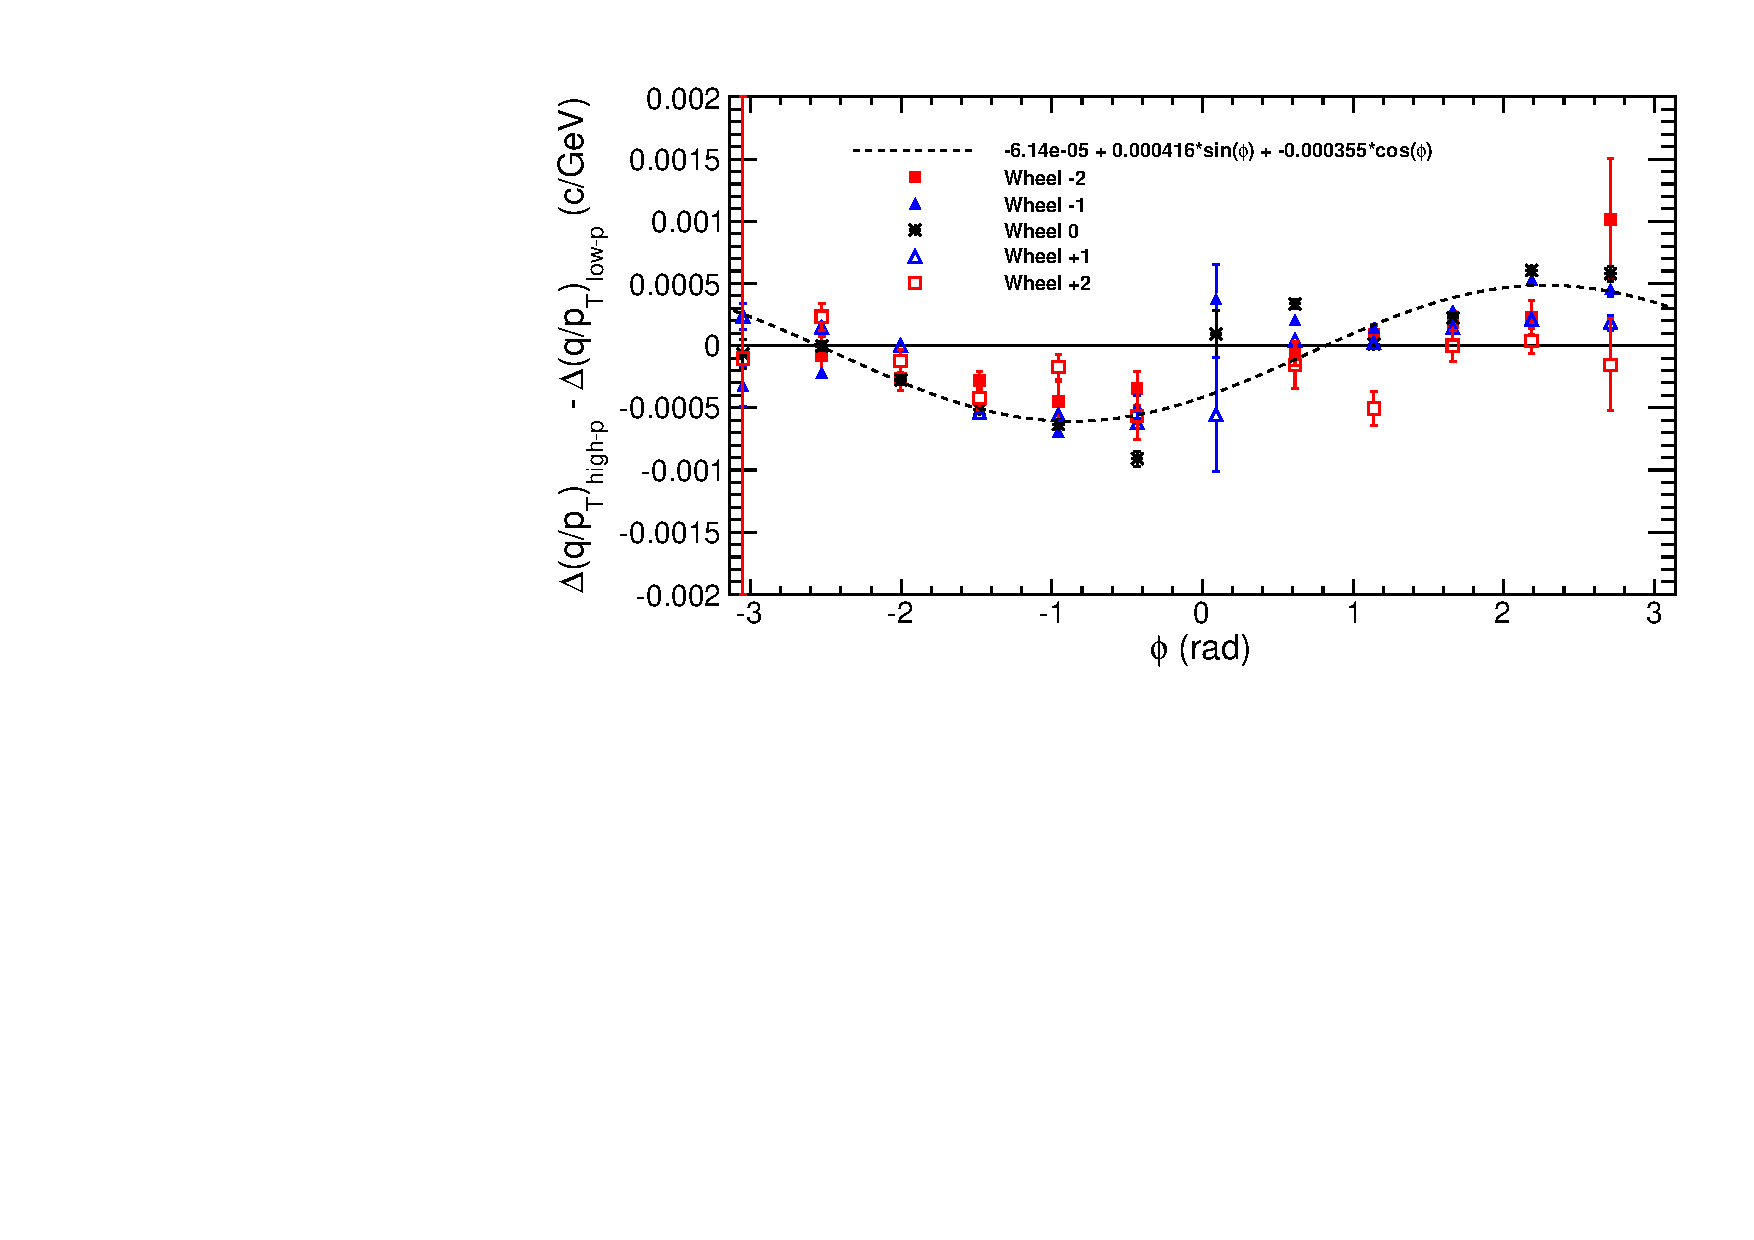
\includegraphics[width=\linewidth]{deltacurv_vs_phi.pdf}

\column{0.4\linewidth}
\begin{itemize}
\item In these plots, we show how the differences between the tops and
  bottoms of the Gaussians vary in $\phi$, $\theta$
\item Top is from raw residuals $\Delta x$
\item Bottom is from curvatures $\Delta(q/p_T)$
\item $\sin(2\phi) \to \sin(\phi)$ in the transformation is not
  understood, but consistent {\scriptsize (when considering different
    tracker geometries and differences of geometries)}
\end{itemize}
\end{columns}
\end{frame}

\begin{frame}
\frametitle{{\large Parameterization and combined fit}}
\framesubtitle{using the $\Delta(q/p_T)$ plots and expanding the expression to include wheels}

$(A)\kappa + \big[(F + F_{\theta}\cot\theta) + $

\hfill $(S + S_{\theta}\cot\theta)\sin(\phi) + (C + C_{\theta}\cot\theta)\cos(\phi)\big]\exp(-\kappa^2 W^2 / 2)$

\begin{center}
$\chi^2/N_{dof} = 2194/1066 = 2.06$
\end{center}
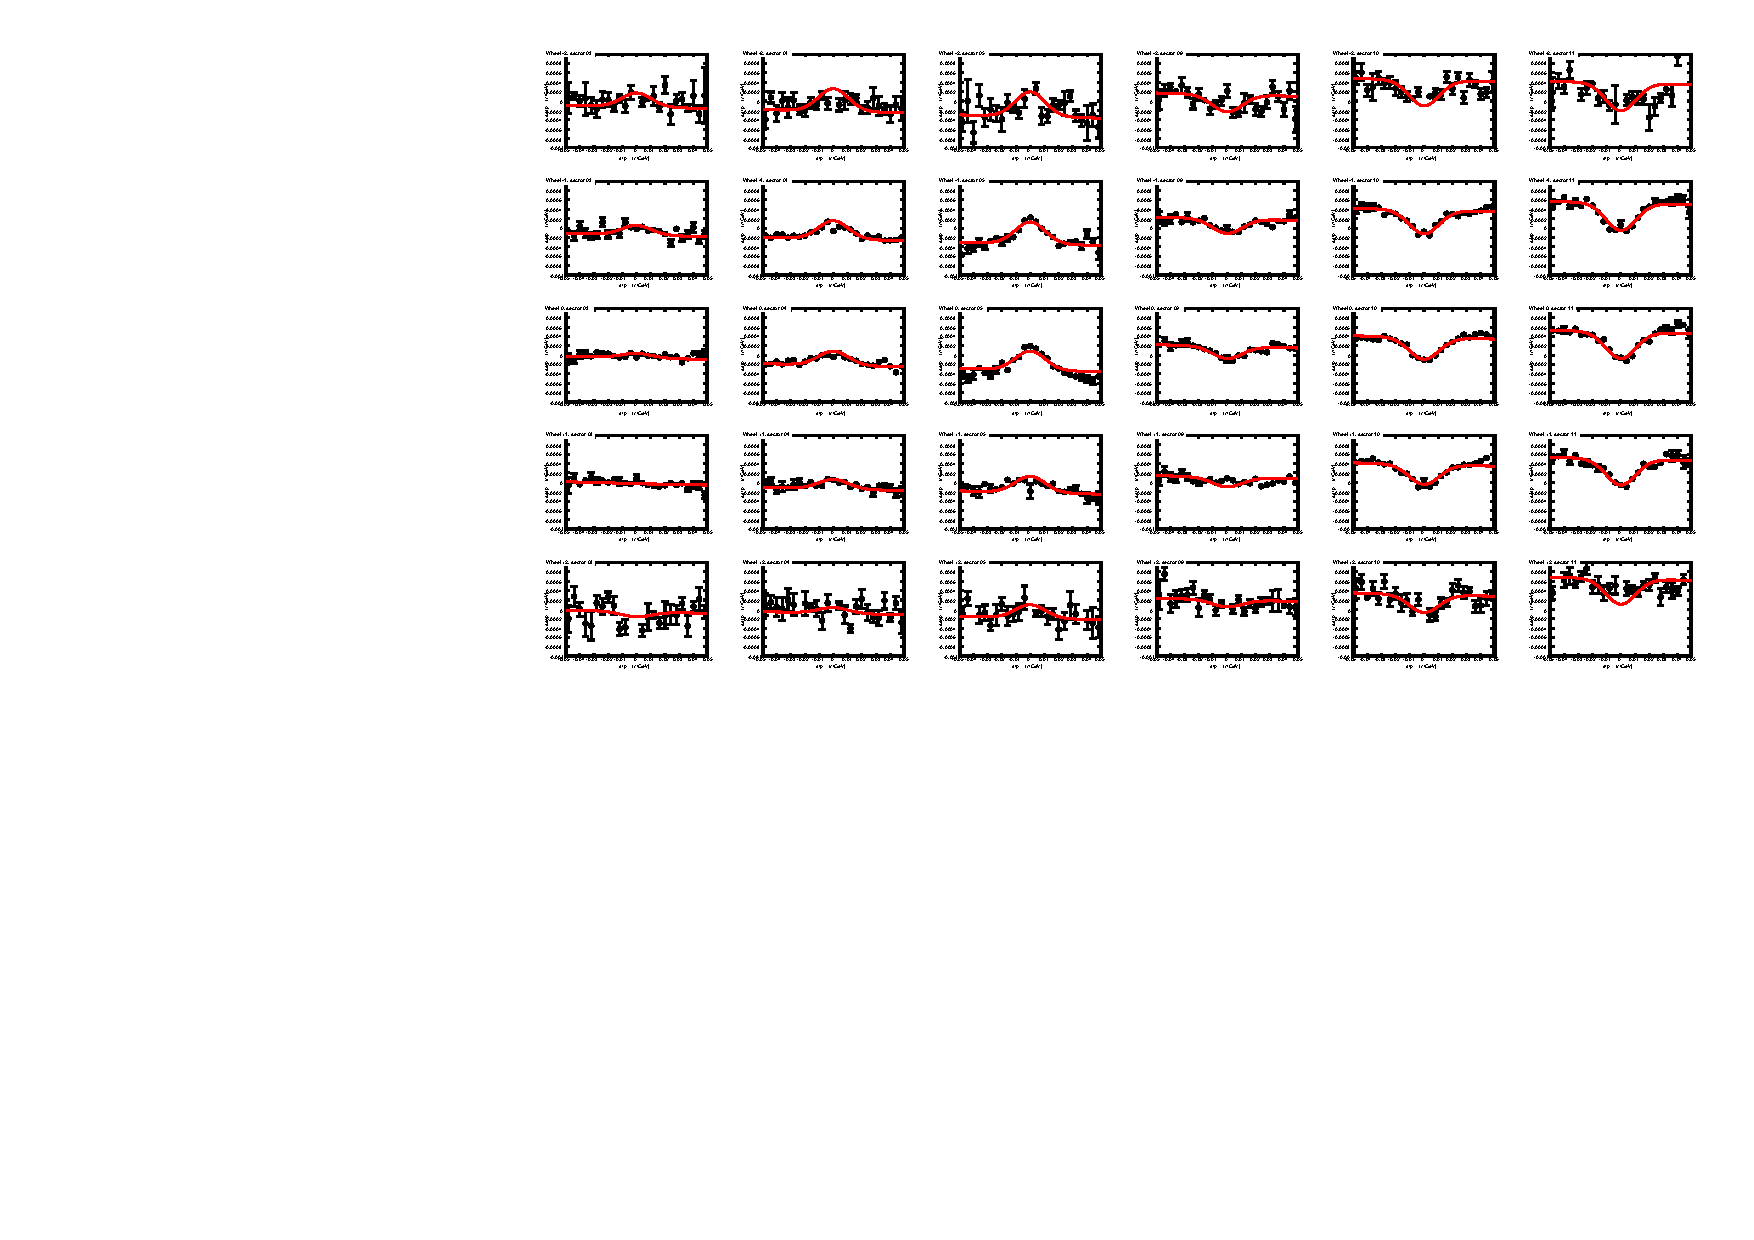
\includegraphics[width=0.9\linewidth]{allfits.pdf}
\end{frame}

\begin{frame}
\frametitle{{\large Millepede-generated mode} {\normalsize (M.~Stoye)}}

\begin{columns}
\column{0.6\linewidth}
\begin{columns}
\column{0.5\linewidth}
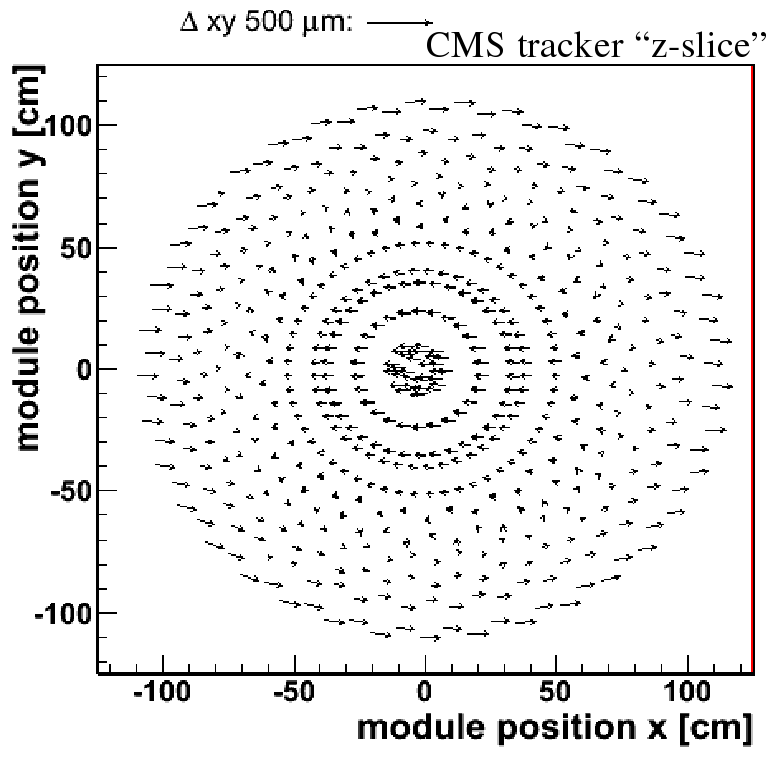
\includegraphics[width=\linewidth]{stoye_deformation.png}
\column{0.5\linewidth}
\only<1>{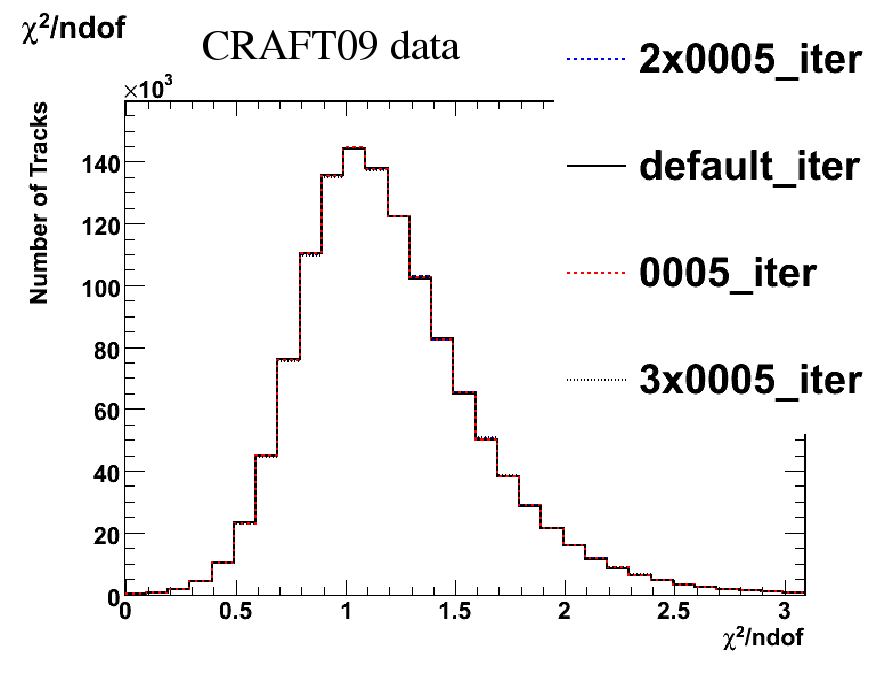
\includegraphics[width=\linewidth]{chi2_invariance.png}}
\only<2>{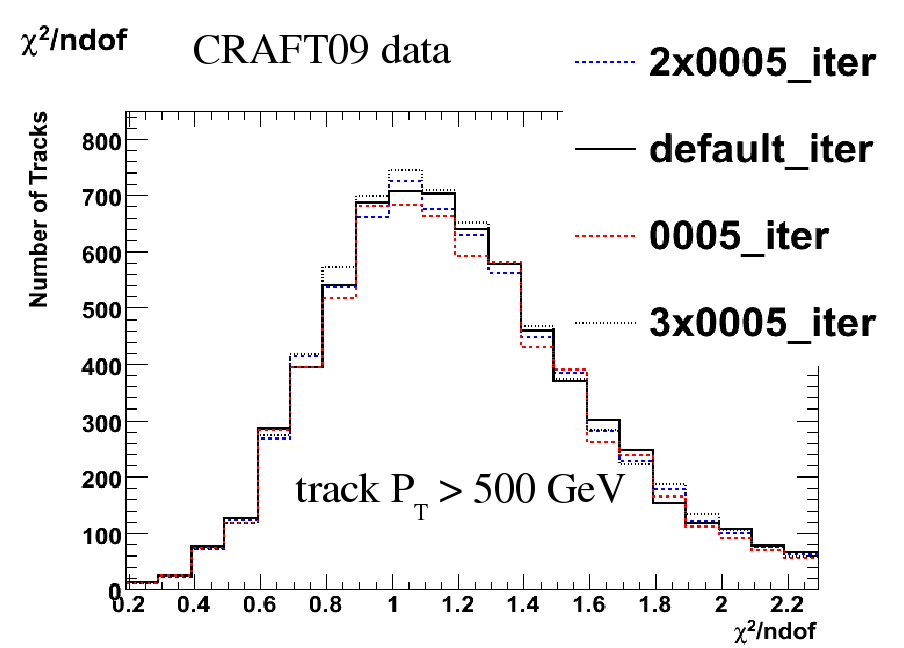
\includegraphics[width=\linewidth]{chi2_invariance_highpt.png}}
\end{columns}

\column{0.4\linewidth}
\begin{itemize}
\item Coherent distortion of tracker with no tracker $\chi^2$ sensitivity

\item We can see its effect with muon reisduals
\end{itemize}
\end{columns}

\vfill
\scriptsize

$(A)\kappa + \big[(F + F_{\theta}\cot\theta) + (S + S_{\theta}\cot\theta)\sin(\phi) + (C + C_{\theta}\cot\theta)\cos(\phi)\big]\exp(-\kappa^2 W^2 / 2)$

\vfill

\begin{tabular}{l r r r r}
 & $\chi^2/N_{dof}$ & $A$\hspace{0.35 cm} & $F$ (GeV$^{-1}$) & $F_{\theta}$ (GeV$^{-1}$) \\\hline
mode$\times$0 & 2194/1066 & $-0.000\,70$ & $-0.000\,082$ & $-0.000\,039$ \\
mode$\times$1 & 2171/1068 & $-0.000\,63$ & $0.000\,098$ & $-0.000\,063$  \\
mode$\times$3 & 1991/942 & $-0.000\,68$ & $0.000\,277$ & $-0.000\,070$ \\\hline
uncertainty & & $0.000\,09$ & $0.000\,005$ & $0.000\,009$ \\
\end{tabular}

\vfill
\hfill \begin{tabular}{l r r r r r}
& $S$ (GeV$^{-1}$) & $S_{\theta}$ (GeV$^{-1}$) & $C$ (GeV$^{-1}$) & $C_{\theta}$ (GeV$^{-1}$) & $W$ (GeV) \\\hline
mode$\times$0 & $0.000\,3533$ & $-0.000\,113$ & $-0.000\,345$ & $-0.000\,057$ & $95.0$ \\
mode$\times$1 & $0.000\,3892$ & $-0.000\,156$ & $-0.000\,335$ & $-0.000\,063$ & $93.1$ \\
mode$\times$3 & $0.000\,4310$ & $-0.000\,170$ & $-0.000\,386$ & $-0.000\,096$ & $84.1$ \\\hline
uncertainty & $0.000\,0064$ & $0.000\,011$ & $0.000\,010$ & $0.000\,016$ & 2.1 \\
\end{tabular}
\end{frame}

\begin{frame}
\frametitle{Graphical presentation}

\scriptsize

$(A)\kappa + \big[(F + F_{\theta}\cot\theta) + (S + S_{\theta}\cot\theta)\sin(\phi) + (C + C_{\theta}\cot\theta)\cos(\phi)\big]\exp(-\kappa^2 W^2 / 2)$

\vfill

\begin{tabular}{l r r r r}
 & $\chi^2/N_{dof}$ & $A$\hspace{0.35 cm} & $F$ (GeV$^{-1}$) & $F_{\theta}$ (GeV$^{-1}$) \\\hline
mode$\times$0 & 2194/1066 & $-0.000\,70$ & $-0.000\,082$ & $-0.000\,039$ \\
mode$\times$1 & 2171/1068 & $-0.000\,63$ & $0.000\,098$ & $-0.000\,063$  \\
mode$\times$3 & 1991/942 & $-0.000\,68$ & $0.000\,277$ & $-0.000\,070$ \\\hline
uncertainty & & $0.000\,09$ & $0.000\,005$ & $0.000\,009$ \\
\end{tabular}

\vfill
\hfill \begin{tabular}{l r r r r r}
& $S$ (GeV$^{-1}$) & $S_{\theta}$ (GeV$^{-1}$) & $C$ (GeV$^{-1}$) & $C_{\theta}$ (GeV$^{-1}$) & $W$ (GeV) \\\hline
mode$\times$0 & $0.000\,3533$ & $-0.000\,113$ & $-0.000\,345$ & $-0.000\,057$ & $95.0$ \\
mode$\times$1 & $0.000\,3892$ & $-0.000\,156$ & $-0.000\,335$ & $-0.000\,063$ & $93.1$ \\
mode$\times$3 & $0.000\,4310$ & $-0.000\,170$ & $-0.000\,386$ & $-0.000\,096$ & $84.1$ \\\hline
uncertainty & $0.000\,0064$ & $0.000\,011$ & $0.000\,010$ & $0.000\,016$ & 2.1 \\
\end{tabular}

\begin{center}
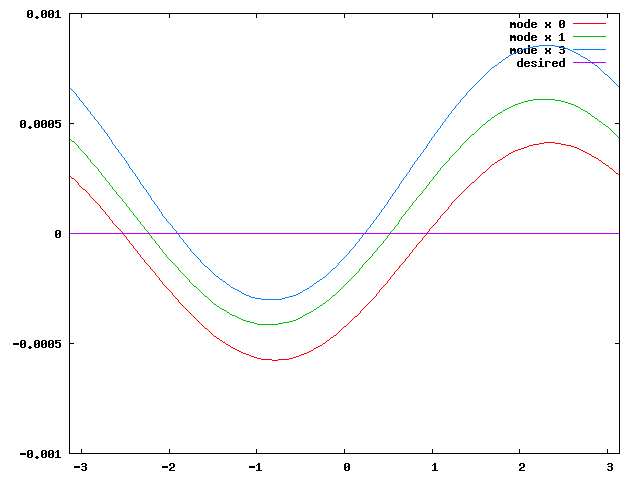
\includegraphics[width=0.4\linewidth]{modes.png}
\end{center}
\end{frame}

\begin{frame}
\frametitle{How it can be used}

\begin{itemize}
\item The observed bias must be corrected in the geometry, {\it even} if
  only to verify that the diagnostic is being correctly interpreted

\item However, {\it uncertainties} on fitted parameters quantify systematic
  errors in momentum for physics analyses

\item Covariance matrix for fit on previous page:

\end{itemize}

{\scriptsize
$(A)\kappa + \big[(F + F_{\theta}\cot\theta) + (S + S_{\theta}\cot\theta)\sin(\phi) + (C + C_{\theta}\cot\theta)\cos(\phi)\big]\exp(-\kappa^2 W^2 / 2)$}

\vspace{0.2 cm}
{\mbox{\hspace{-1 cm}}\begin{minipage}{1.2\linewidth}
\tiny $\begin{array}{r r r r r r r r}
7.2\cdot 10^{-9} &  1.9\cdot 10^{-11} &  5.1\cdot 10^{-12} &  -8.3\cdot 10^{-12} &  -1.7\cdot 10^{-11} &  -6.4\cdot 10^{-11} &  4.5\cdot 10^{-11} &  -1.2\cdot 10^{-6} \\
&  2.9\cdot 10^{-11} &  -1.2\cdot 10^{-12} &  3.2\cdot 10^{-12} &  4\cdot 10^{-12} &  1.4\cdot 10^{-13} &  1.8\cdot 10^{-12} &  1\cdot 10^{-8} \\
&  &  8.2\cdot 10^{-11} &  3.8\cdot 10^{-12} &  1\cdot 10^{-11} &  2.2\cdot 10^{-12} &  -4.9\cdot 10^{-12} &  -2.4\cdot 10^{-7} \\
&  &  &  4.1\cdot 10^{-11} &  -2.9\cdot 10^{-12} &  1.9\cdot 10^{-12} &  6.6\cdot 10^{-12} &  1.8\cdot 10^{-6} \\
&  &  &  &  1.2\cdot 10^{-10} &  6.2\cdot 10^{-12} &  -1\cdot 10^{-11} &  -1.7\cdot 10^{-6} \\
&  &  &  &  &  9.7\cdot 10^{-11} &  -4.6\cdot 10^{-12} &  8.2\cdot 10^{-7} \\
&  &  &  &  &  &  2.6\cdot 10^{-10} &  2.5\cdot 10^{-6} \\
&  &  &  &  &  &  &  4.4 \\
\end{array}$
\end{minipage}}

\begin{itemize}

\item Regardless of any remaining global distortions of the tracker,
  we would have measured limits on how wrong the momenta might be

\item Precision with CRAFT-09: a few percent momentum uncertainty at
  1~TeV (depending on parameterization; 0.5\% for simple constant)
\end{itemize}
\end{frame}

\begin{frame}
\frametitle{{\large What this says about charge ratio}}

\begin{columns}
\column{0.7\linewidth}
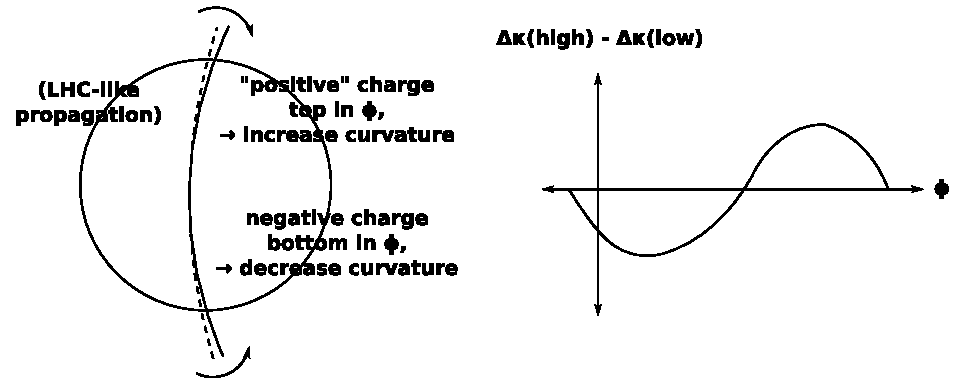
\includegraphics[width=\linewidth]{impact_on_charge_ratio.pdf}

\column{0.3\linewidth}
\begin{itemize}
\item Shape of the effect has maximum effect on cosmic rays and resonances decaying at rest
\end{itemize}
\end{columns}

\begin{itemize}
\item Top and bottom are both affected by $0.000\,5$~GeV$^{-1}$ \\ $\to$ 50\% at 1~TeV or 0.05\% at 1~GeV

\item But there's a fundamental uncertainty here: we measure
  $\Delta \kappa(\mbox{high}) - \Delta \kappa(\mbox{low})$ where ``high''
  momentum tracks have \mbox{$p_T \gg$ 100~GeV,} and ``low'' have \mbox{$p_T \ll$ 100~GeV}

\item From what we know now, either the $Z$ will be unaffected and the
  $Z'$ completely smeared, or vice-versa, or a little of each

\item If we assume that CRAFT-08, CRAFT-09, and the current alignment
  have the same weak modes (not guaranteed), then it seems that the
  $Z'$ will be okay: effect on charge ratio and cosmics endpoint are
  $\sim0.000\,05$~GeV$^{-1}$
\end{itemize}
\end{frame}

\begin{frame}
\frametitle{Absolute curvature bias}
\begin{itemize}
\item If we could know the absolute curvature bias of either high or
  low momentum tracks, we could use the muon residuals to predict
  to the other

\hfill 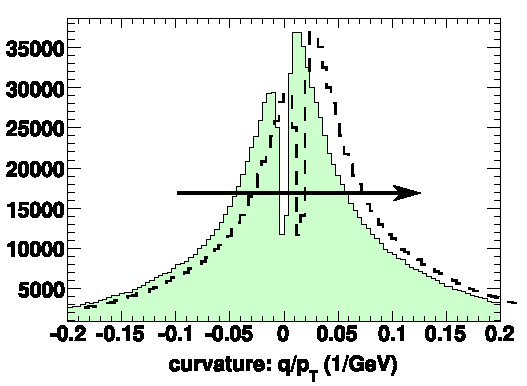
\includegraphics[width=0.4\linewidth]{biases.pdf}

\vspace{-3 cm}
\item Cosmics endpoint: assuming $\sim$flat \\ efficiency for
  high-momentum muons, \\ cosmic ray spectrum in $q/p_T$ must \\ point at
  zero (they trail off to infinite \\ momentum)
\begin{itemize}
\item identifies high-momentum \\ constant offset in $\Delta(q/p_T)$ vs $q/p_T$ (next slide)
\end{itemize}

\item Known resonance masses: identify linear slope in low-momentum $\Delta(q/p_T)$ vs $q/p_T$

\item Curvature of tracks in zero magnetic field: identify constant offset in low-momentum $\Delta(q/p_T)$ vs $q/p_T$

\item $K_S \to \pi^+\pi^-$ decay direction constraint: identify constant offset in low-momentum $\Delta(q/p_T)$ vs $q/p_T$ (following slides)
\end{itemize}
\end{frame}

\begin{frame}
\frametitle{Cosmics endpoint {\normalsize (I.~Furi\'c)}}

\begin{columns}
\column{0.65\linewidth}
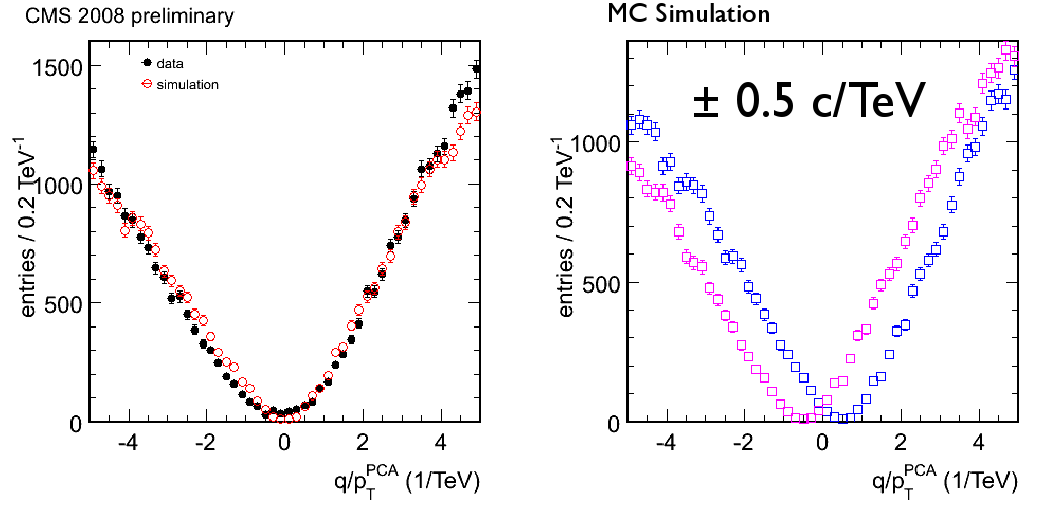
\includegraphics[width=\linewidth]{ivan_cosmic_endpoint.png}

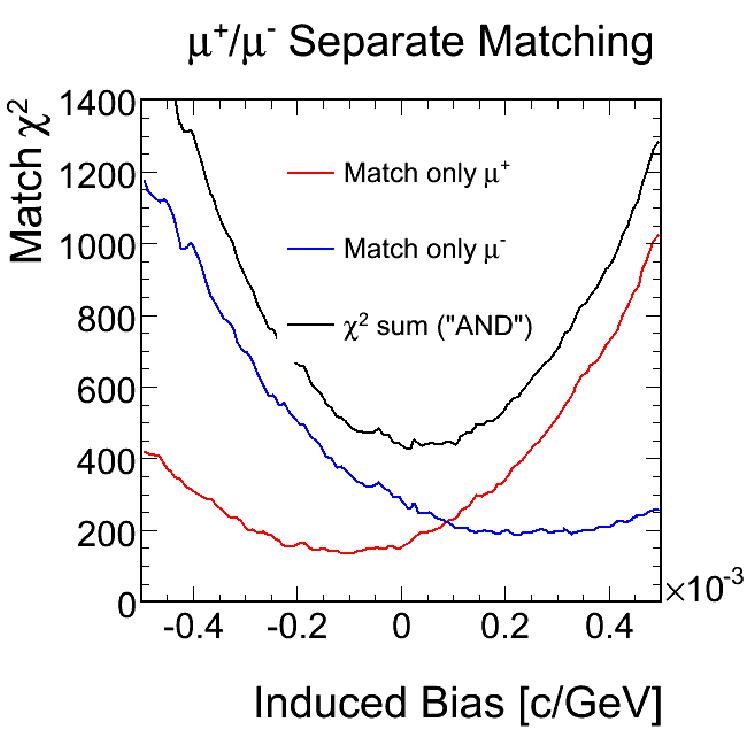
\includegraphics[width=0.7\linewidth]{ivan_chi2.png}
\column{0.5\linewidth}
\begin{itemize}
\item Distribution of cosmic rays trail off at high $p_T$, so positive
  and negative distributions must both point to $q/p_T = 0$ (infinite momentum)

\item Doesn't assume charge ratio, only shape of spectrum (well-known ``energy$^{-2.7}$'')

\item Data are most consistent with $\sim 0.000\,05$~GeV$^{-1}$, ten times
  smaller than $\Delta \kappa(\mbox{high}) - \Delta \kappa(\mbox{low})$ = \\ \hfill $0.000\,5 \sin\phi$~GeV$^{-1}$

\item Implies that the muon-residuals effect is mostly in $\Delta \kappa(\mbox{low})$?  Can we check that?

\end{itemize}
\end{columns}
\end{frame}

\begin{frame}
\frametitle{{\large $K_S \to \pi^+\pi^-$ direction constraint}}

\begin{itemize}
\item Momentum sum of the $\pi^+\pi^-$ system must be collinear with
  the displacement of the secondary vertex

\item As a constraint on momenta, this is orthogonal to resonance mass
\end{itemize}

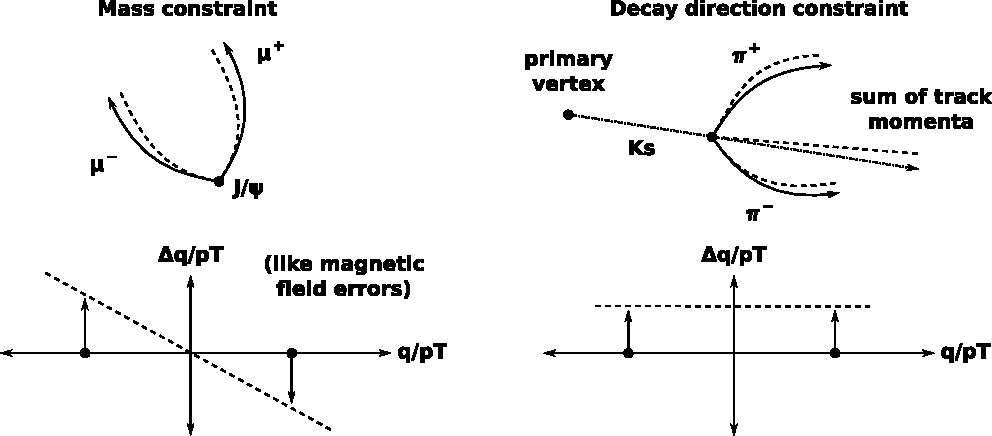
\includegraphics[width=\linewidth]{diagram.pdf}

\begin{itemize}
\item These two are the first terms in a general $\Delta \kappa(\kappa, \phi, \theta)$ expansion in $\kappa$

\end{itemize}
\end{frame}

\begin{frame}
\frametitle{Implementing the $K_S$ constraint}
\framesubtitle{to get a sense of how tight it is from Nov-Dec 2009 data}

\hfill 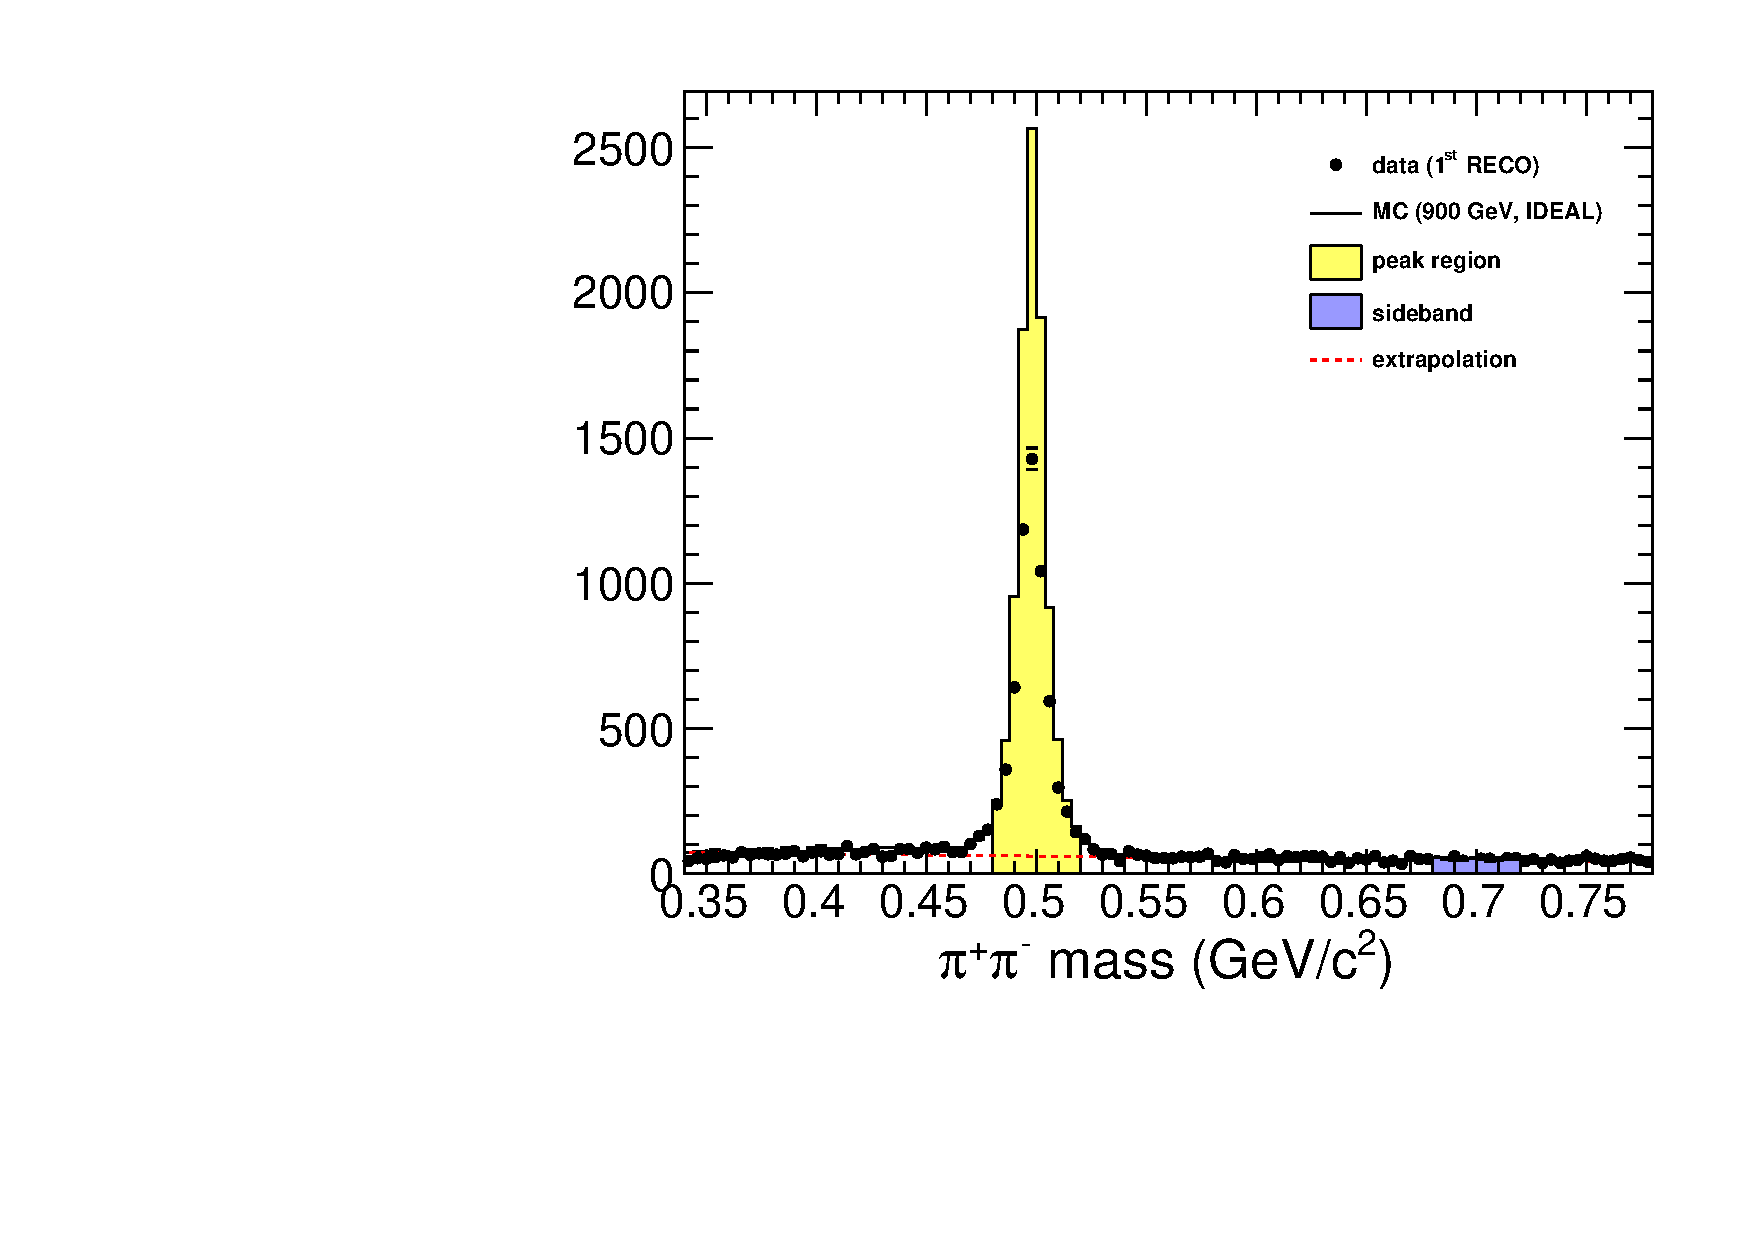
\includegraphics[width=0.5\linewidth]{kaonTracking2_masspeak.pdf}

\vspace{-4.6 cm}
\begin{itemize}
\item Select events using
\begin{itemize}
\item $\pi^+\pi^-$ mass with \\ sideband subtraction
\item vertex inside the first \\ pixel layer
\end{itemize}
\item Pointing to choose the primary \\ vertex in $z$ projection
\end{itemize}

\hspace{1 cm} 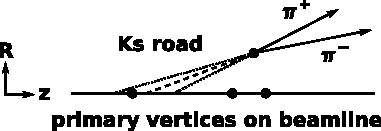
\includegraphics[width=0.3\linewidth]{diagram2.pdf}

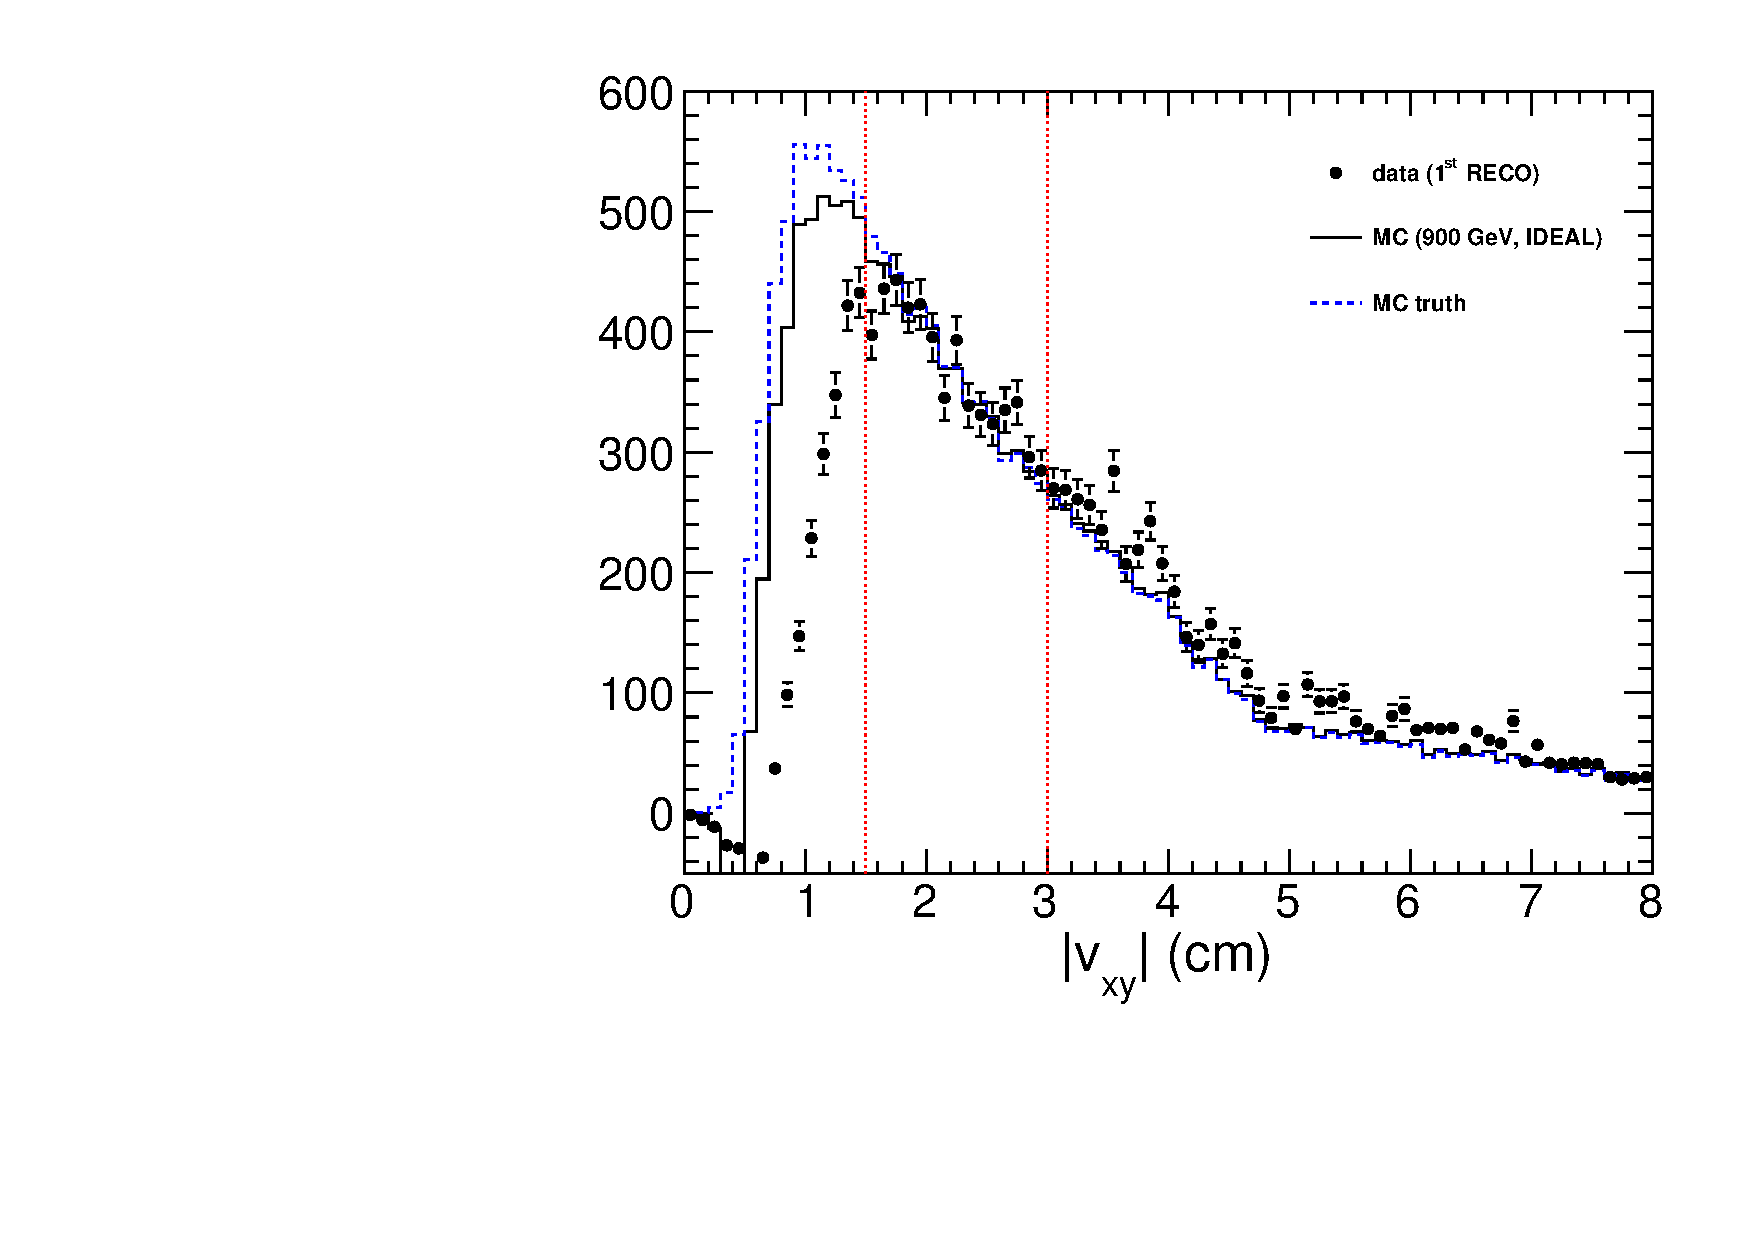
\includegraphics[height=3.5 cm]{kaonTracking2_vxy.pdf}
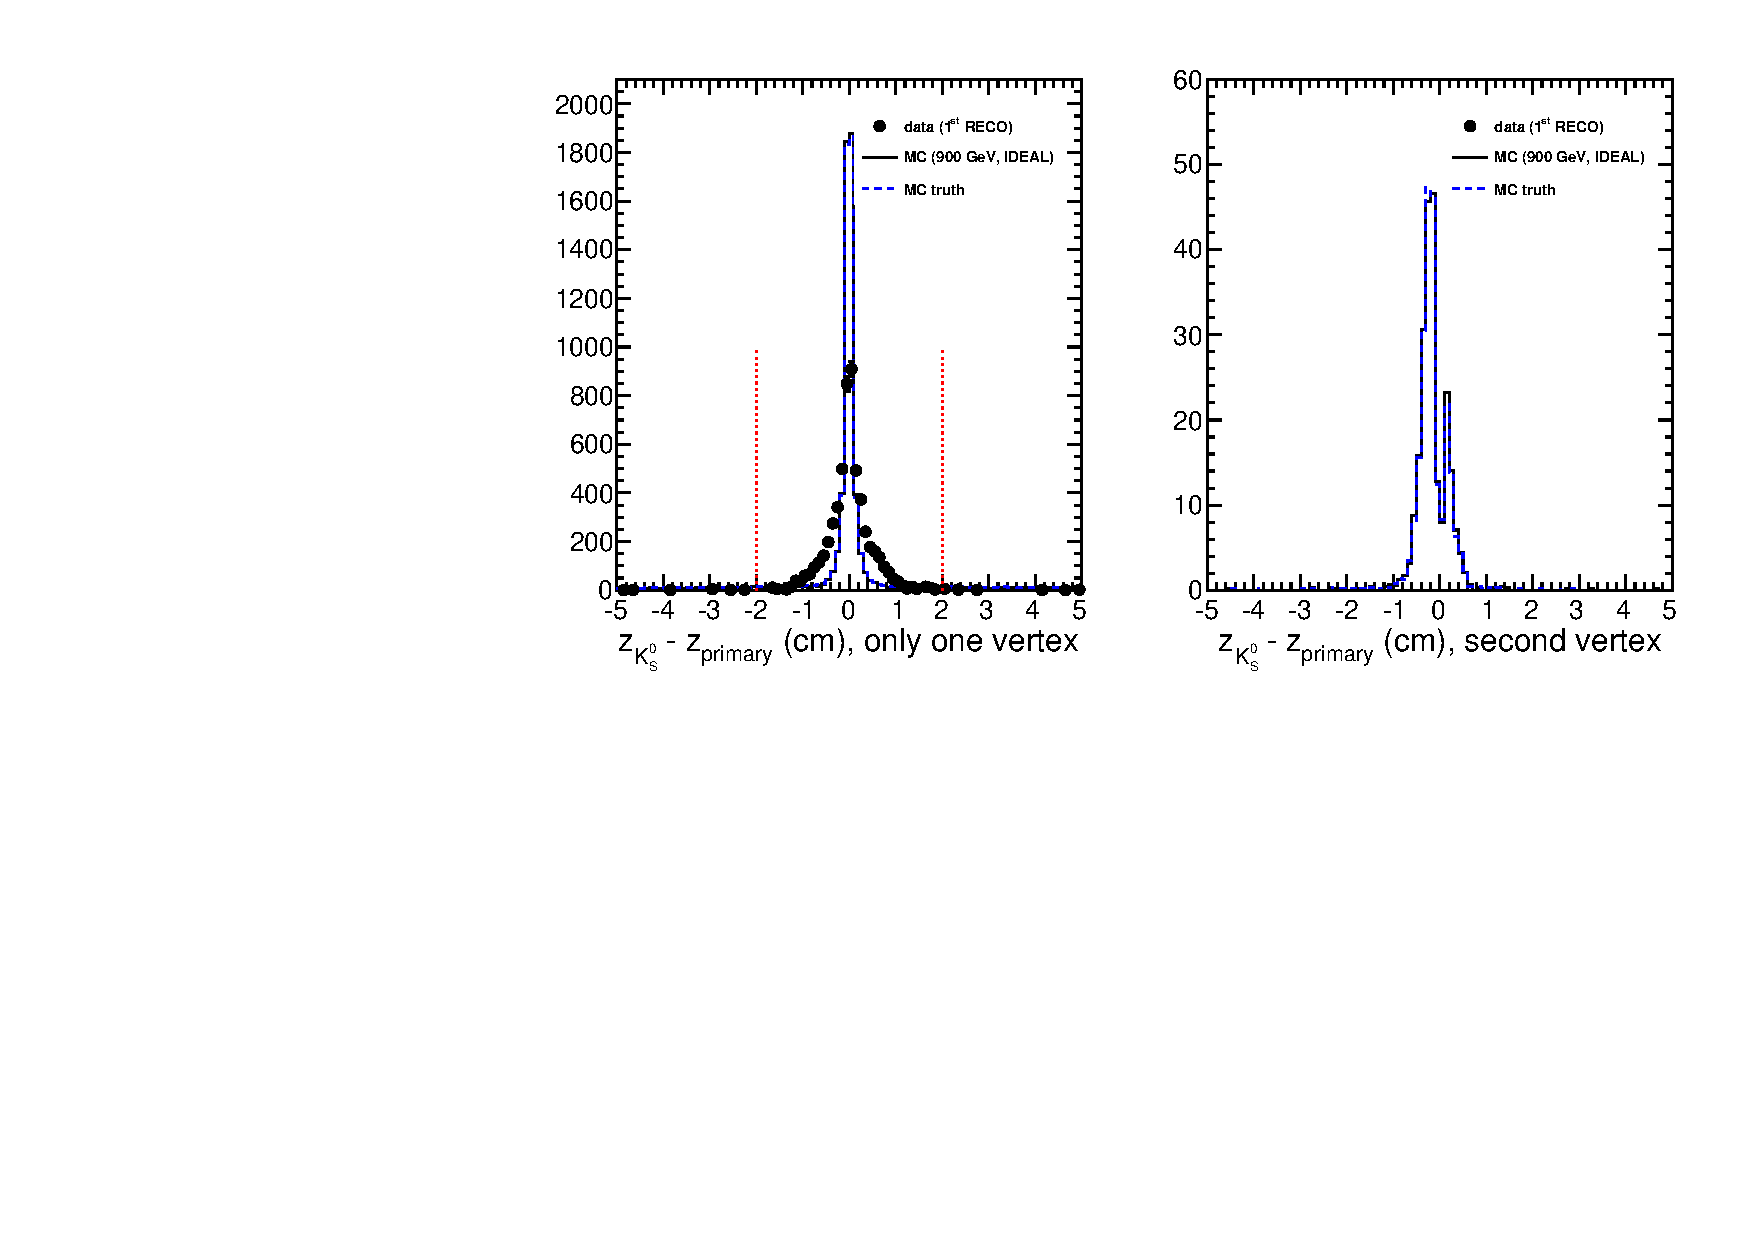
\includegraphics[height=3.5 cm]{kaonTracking2_zcut.pdf}
\end{frame}

\begin{frame}
\frametitle{Observable: $\Delta \phi$}

\begin{itemize}
\item Angle between primary-to-secondary displacement vector and $\pi^+\pi^-$ momentum sum in the transverse plane: $\Delta \phi$

\item Not used up by any selection requirements
\end{itemize}

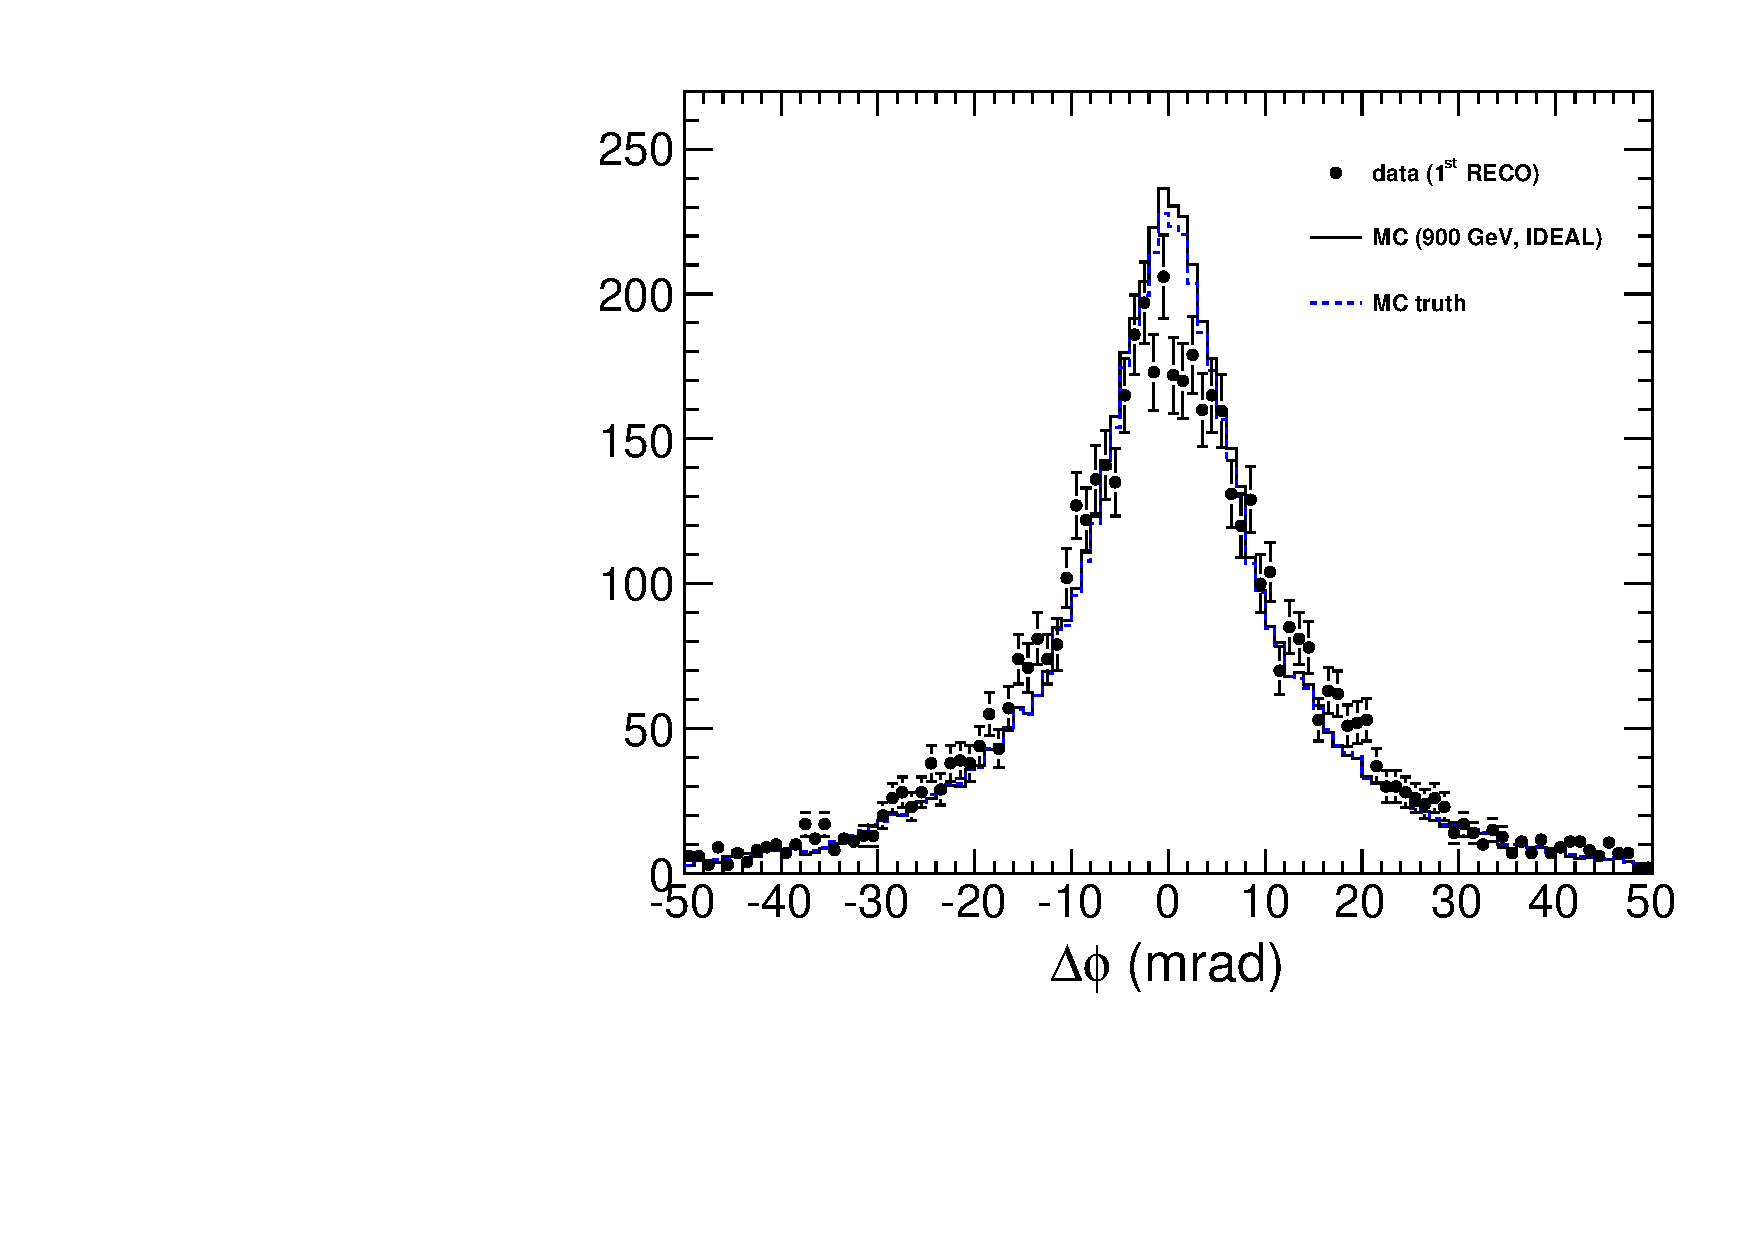
\includegraphics[width=0.5\linewidth]{kaonTracking2_deltaphi.pdf}
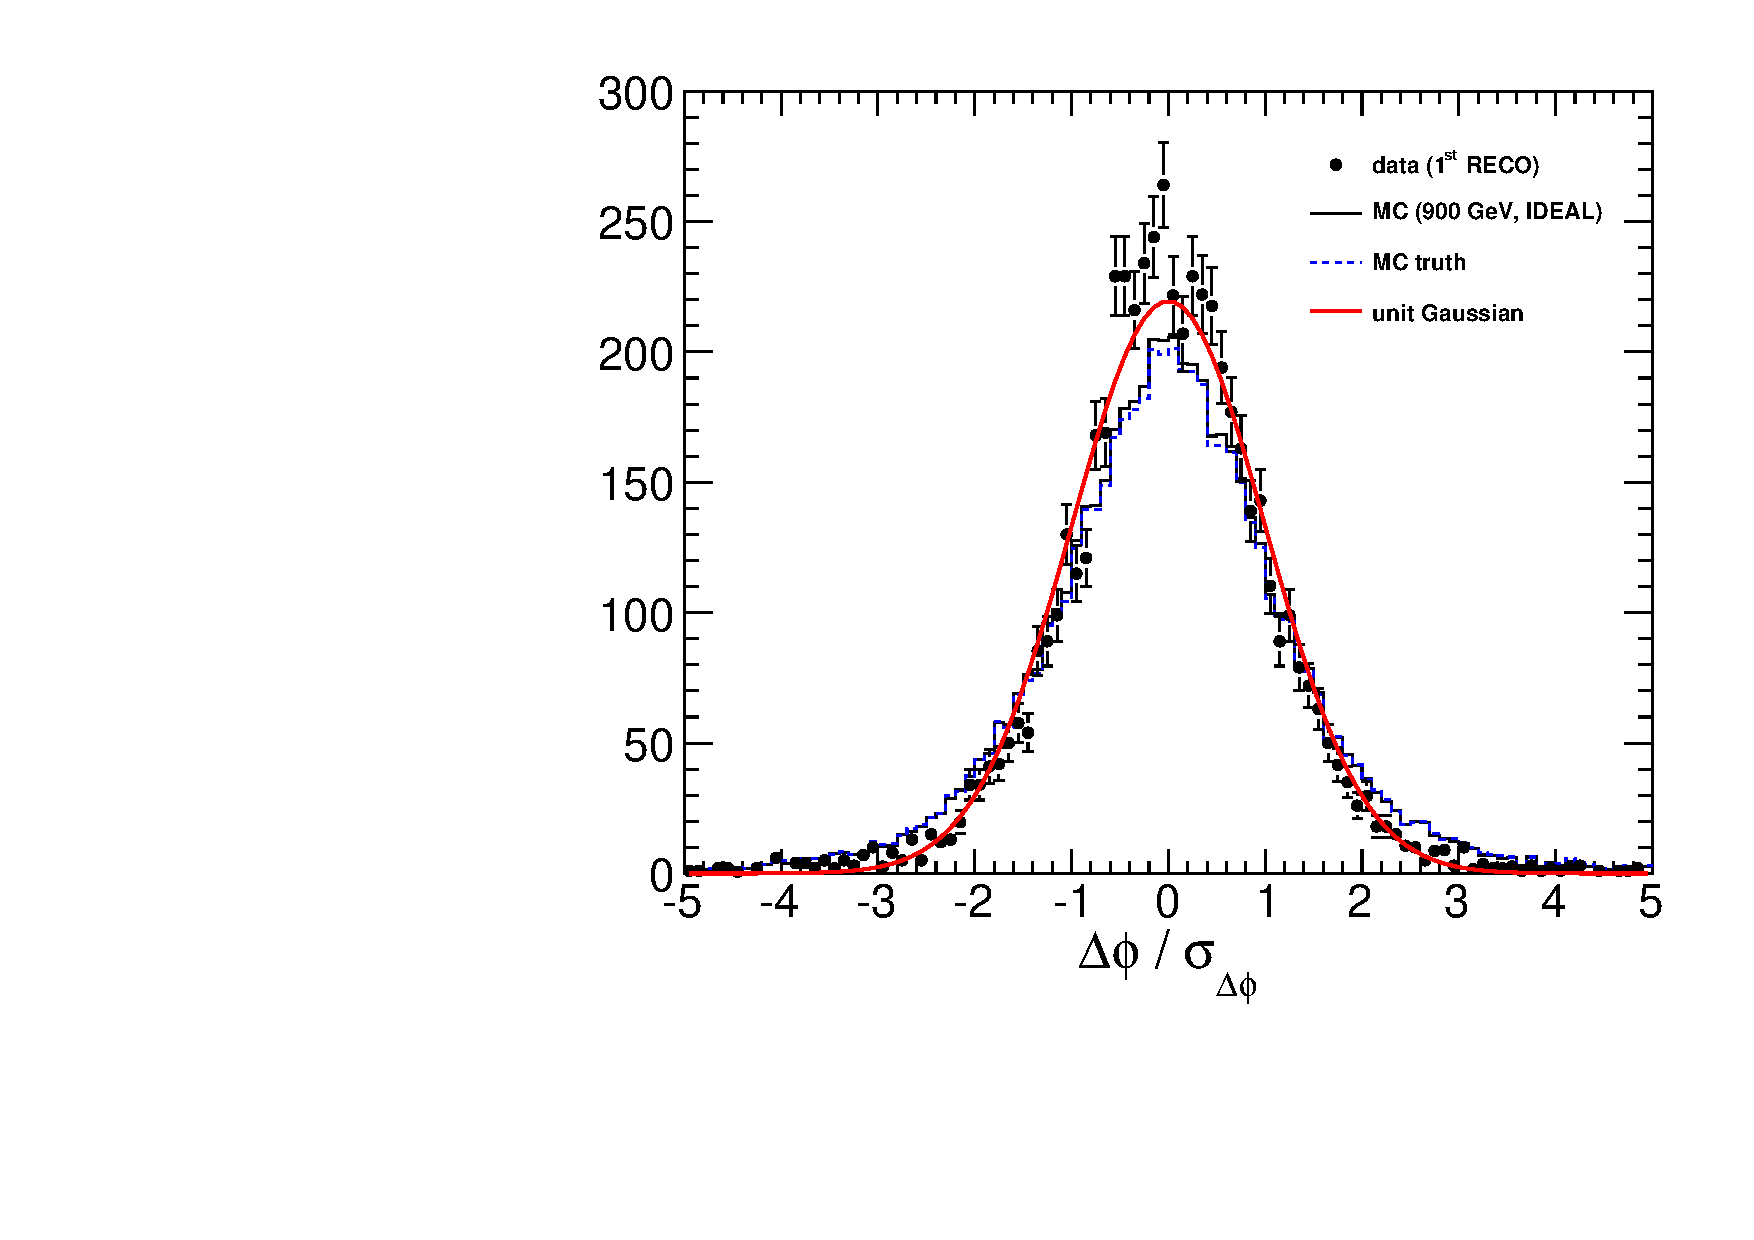
\includegraphics[width=0.5\linewidth]{kaonTracking2_normalized.pdf}

\begin{itemize}
\item No observed bias, with some uncertainty
\end{itemize}
\end{frame}

\begin{frame}
\frametitle{Convert to absolute $\Delta(q/p_T)$}

\begin{itemize}
\item Compute $\frac{\partial \Delta(q/p_T)}{\partial \Delta \phi}$ by taking numerical derivatives with the vertex-fitter
\end{itemize}

\vfill
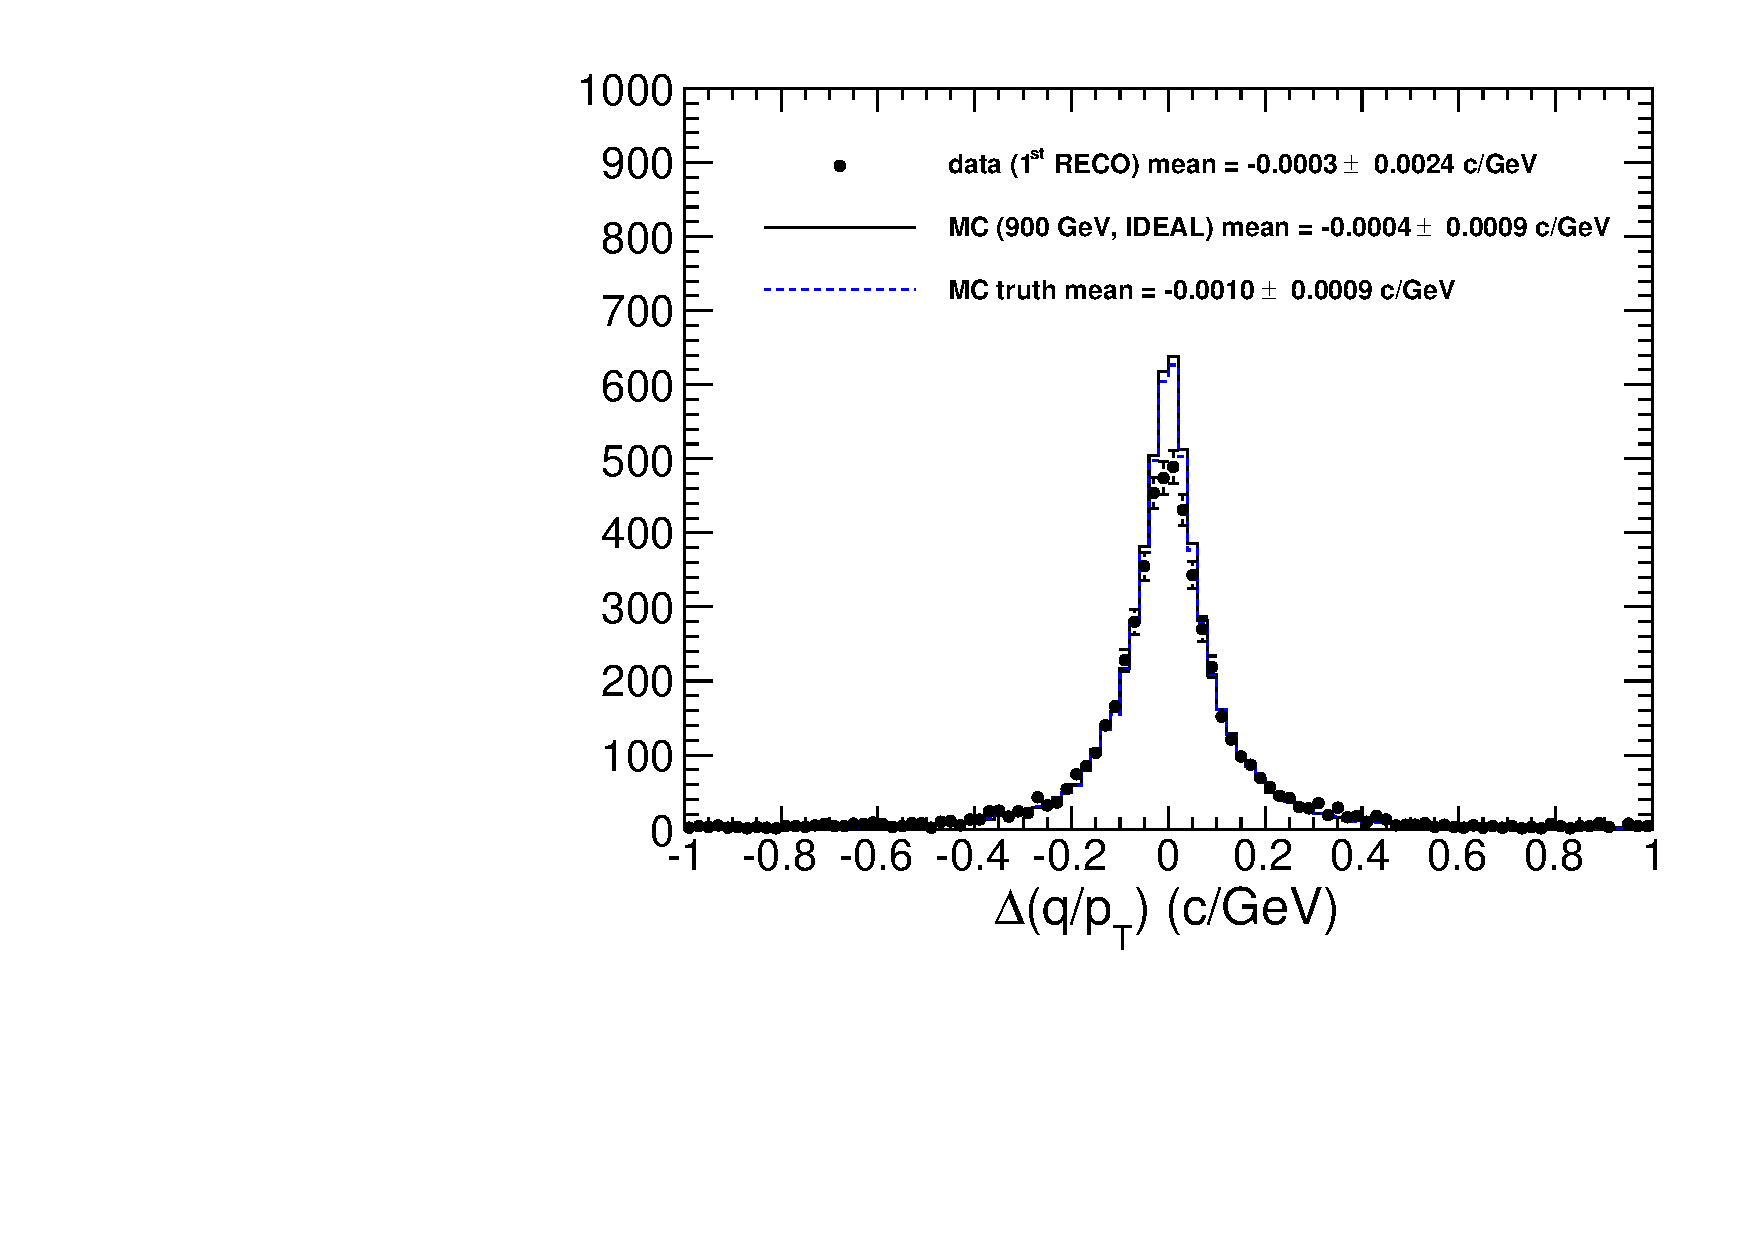
\includegraphics[width=0.5\linewidth]{kaonTracking2_deltaqoverpt.pdf}
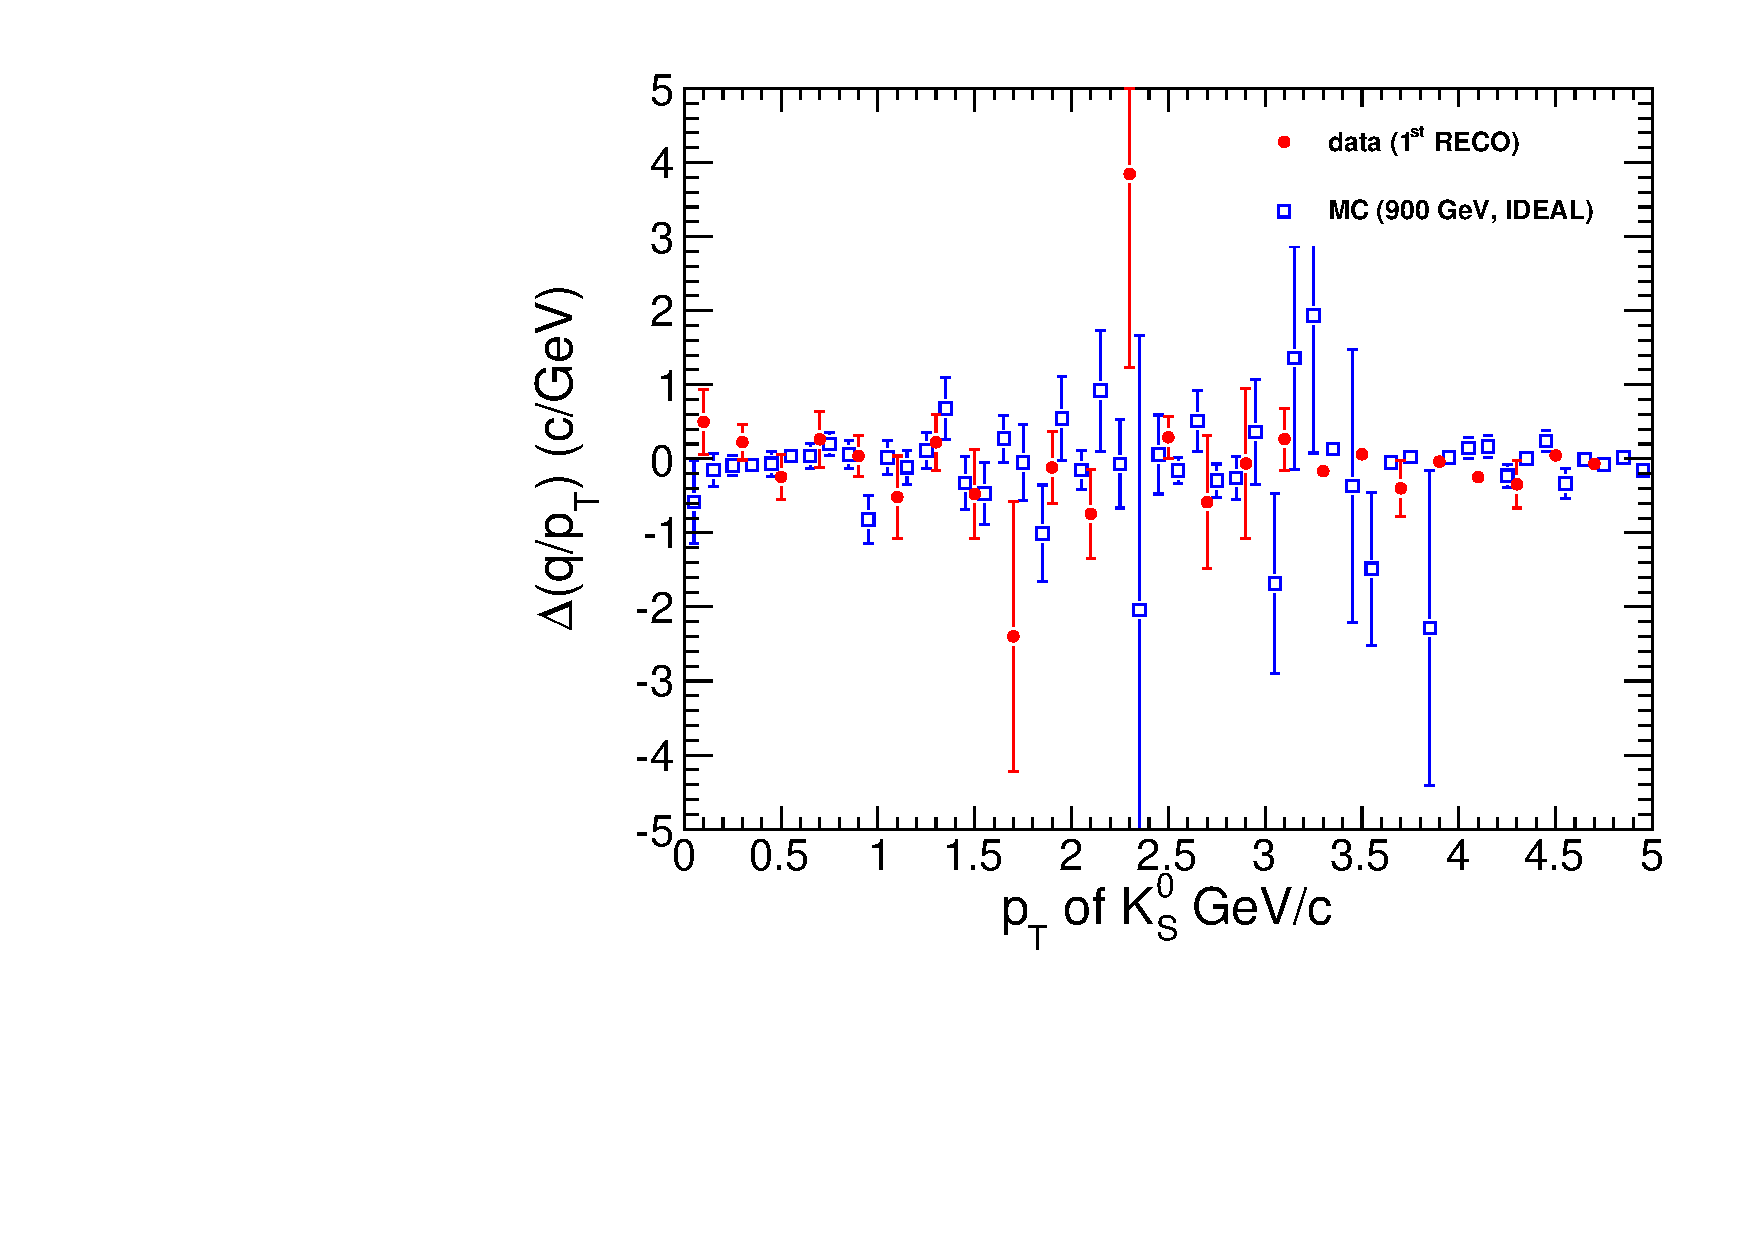
\includegraphics[width=0.5\linewidth]{kaonTracking2_deltaqoverpt_vspt.pdf}

\vfill
\begin{itemize}
\item $\Delta \kappa(\mbox{low}) = -0.000\,3 \pm 0.002\,4$~GeV$^{-1}$
\item 0.24\% uncertainty in bias of 1~GeV tracks
\item Uncertainty in bias of 1~TeV tracks = 240\% (plus a few percent from the $\Delta \kappa(\mbox{high}) - \Delta \kappa(\mbox{low})$ propagation)
\end{itemize}
\end{frame}

\begin{frame}
\frametitle{{\large Flat with respect to everything else}}

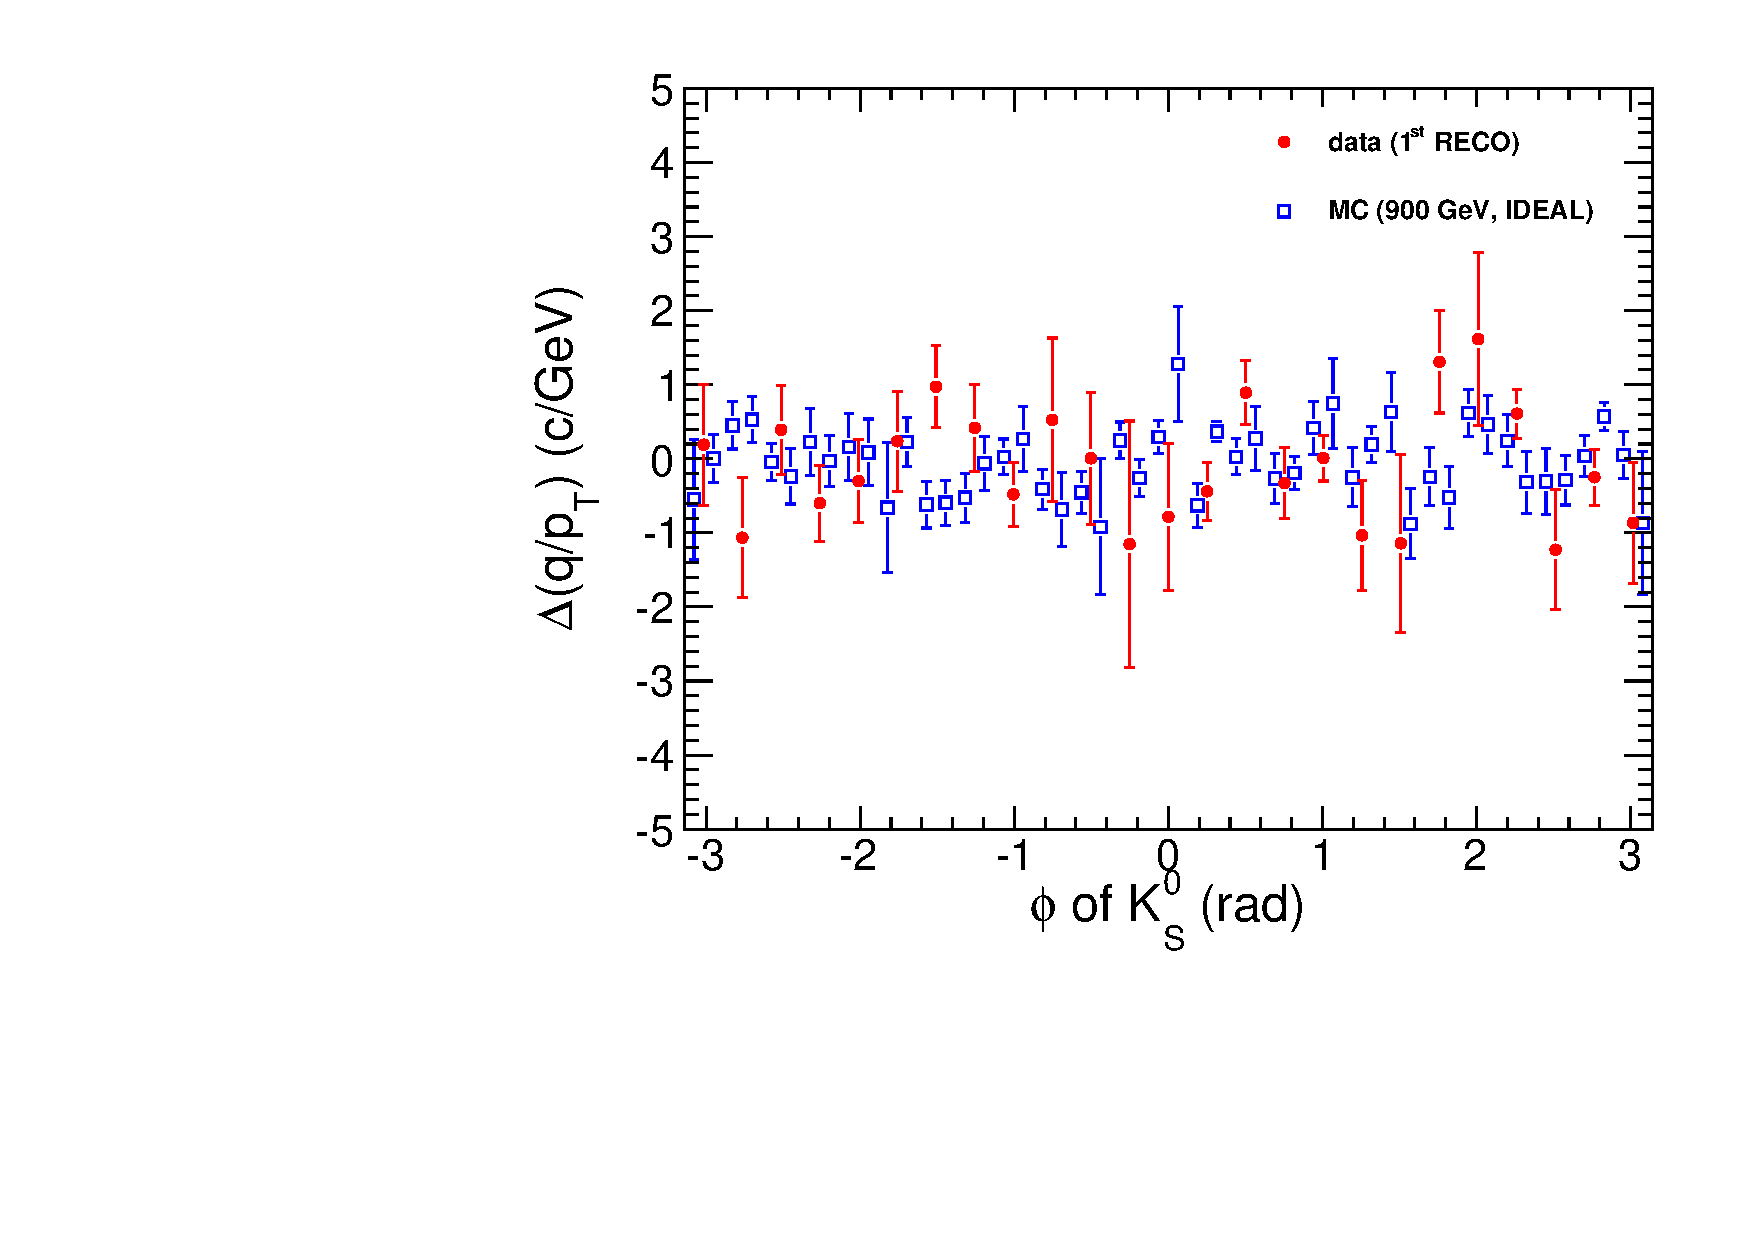
\includegraphics[width=0.32\linewidth]{kaonTracking2_deltaqoverpt_vsphi.pdf}
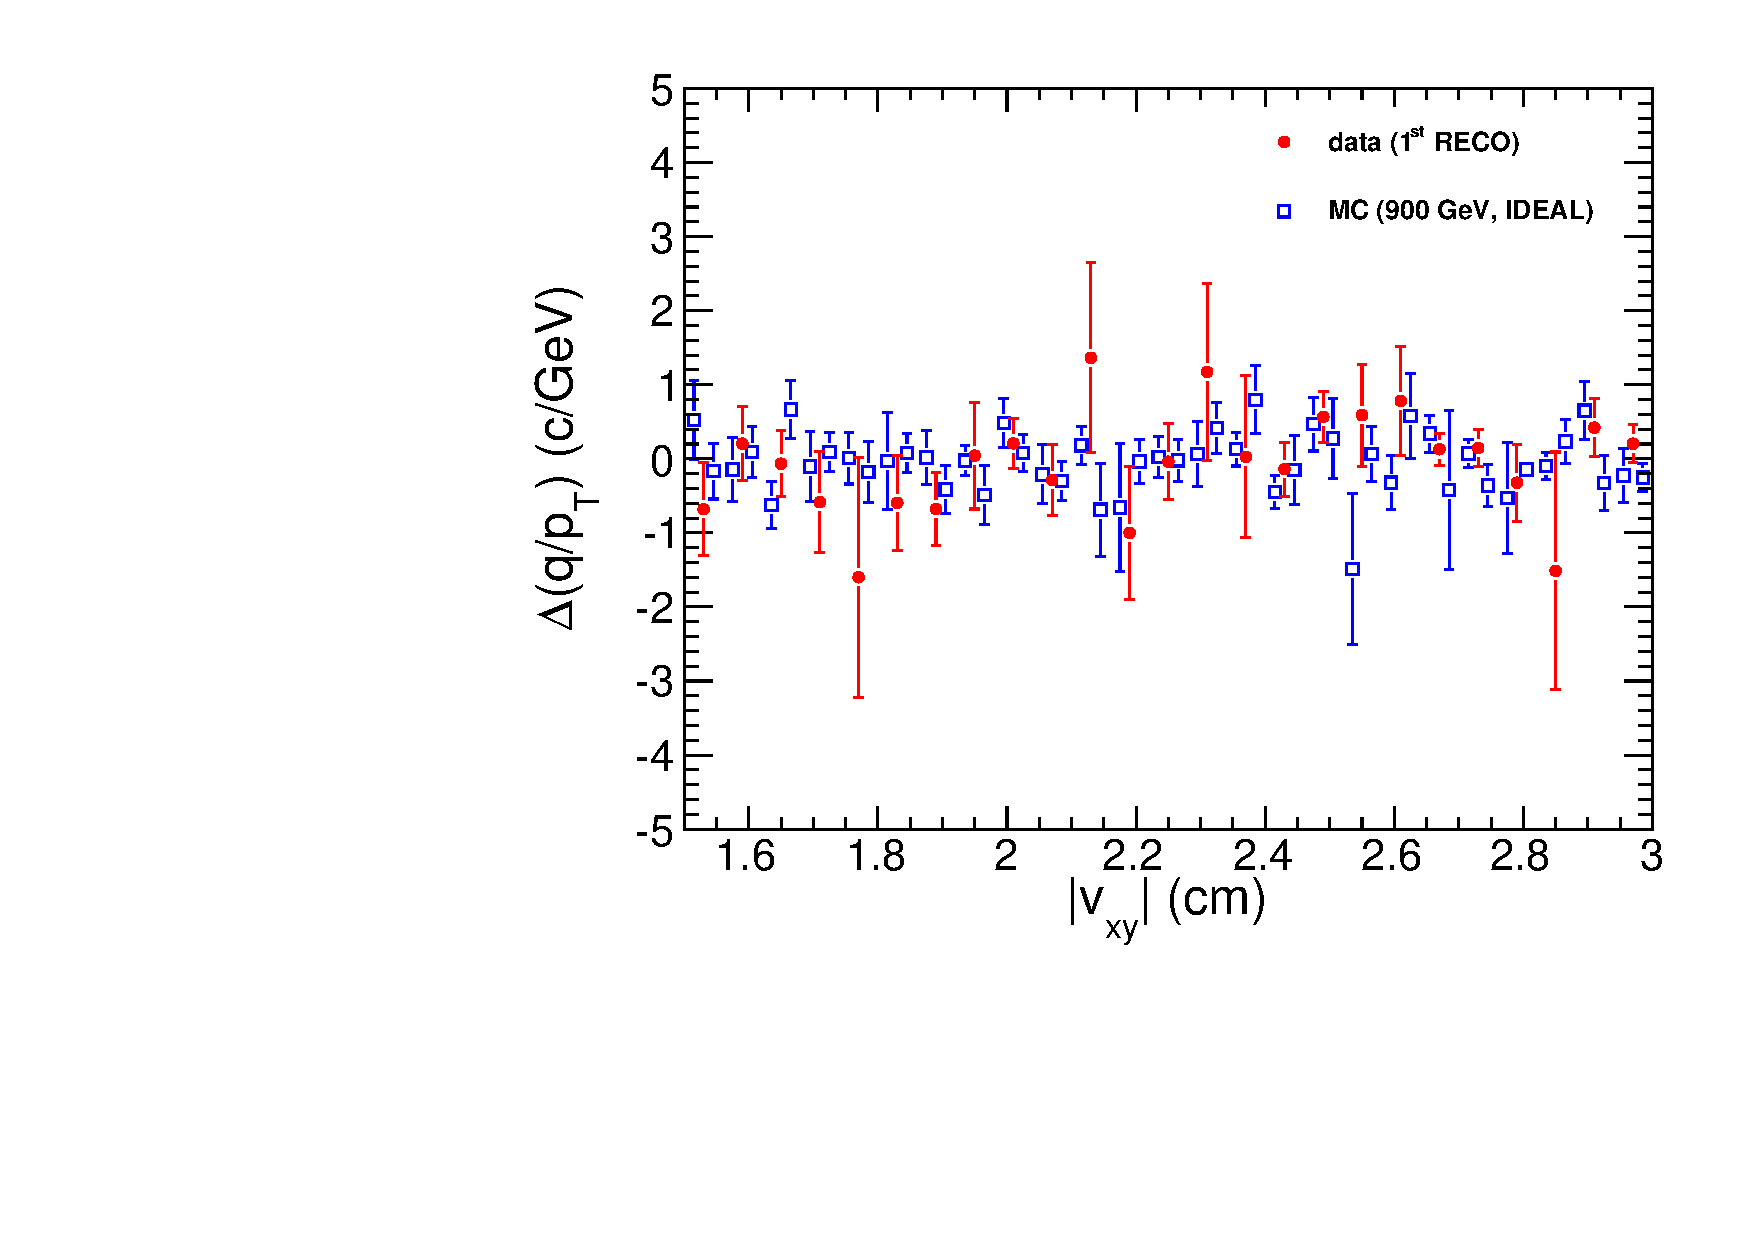
\includegraphics[width=0.32\linewidth]{kaonTracking2_deltaqoverpt_vsvxy.pdf}
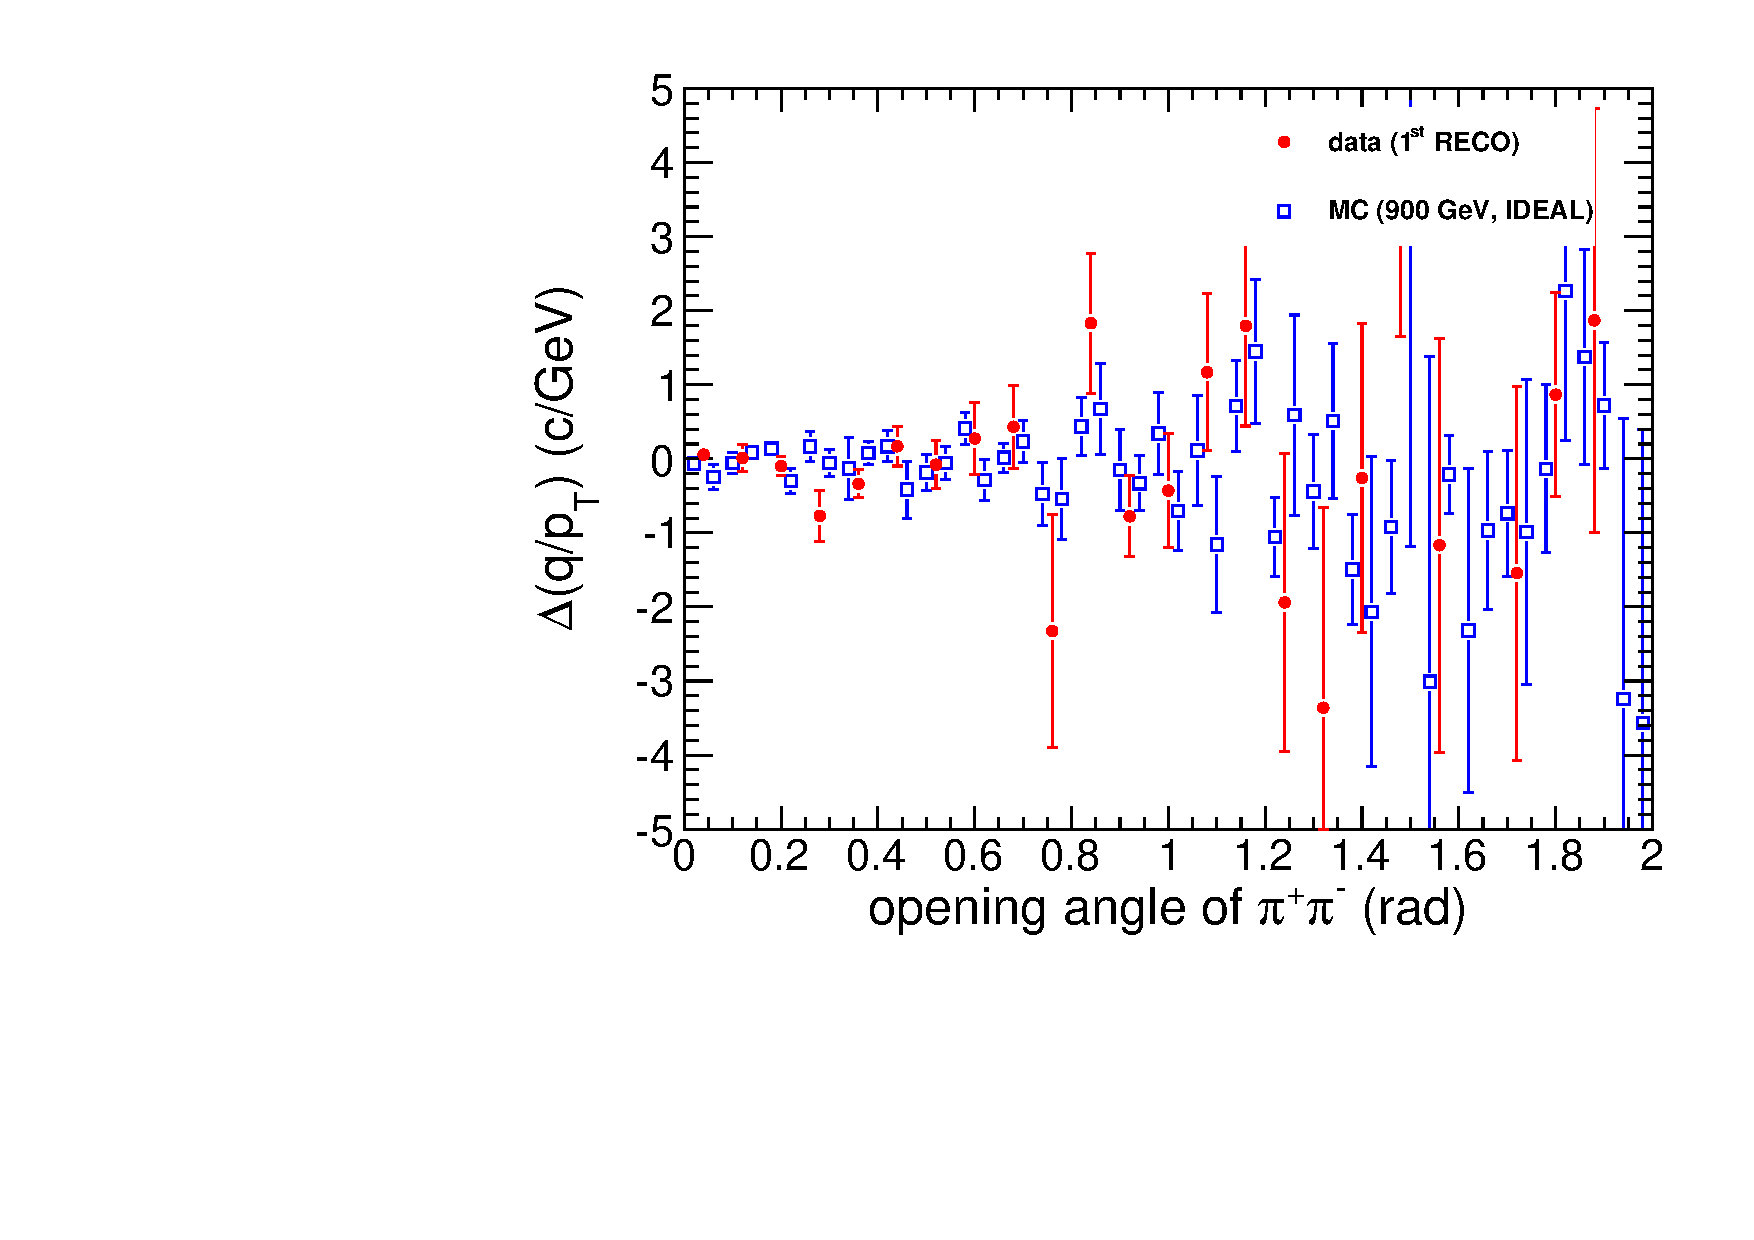
\includegraphics[width=0.32\linewidth]{kaonTracking2_deltaqoverpt_vsopening.pdf}

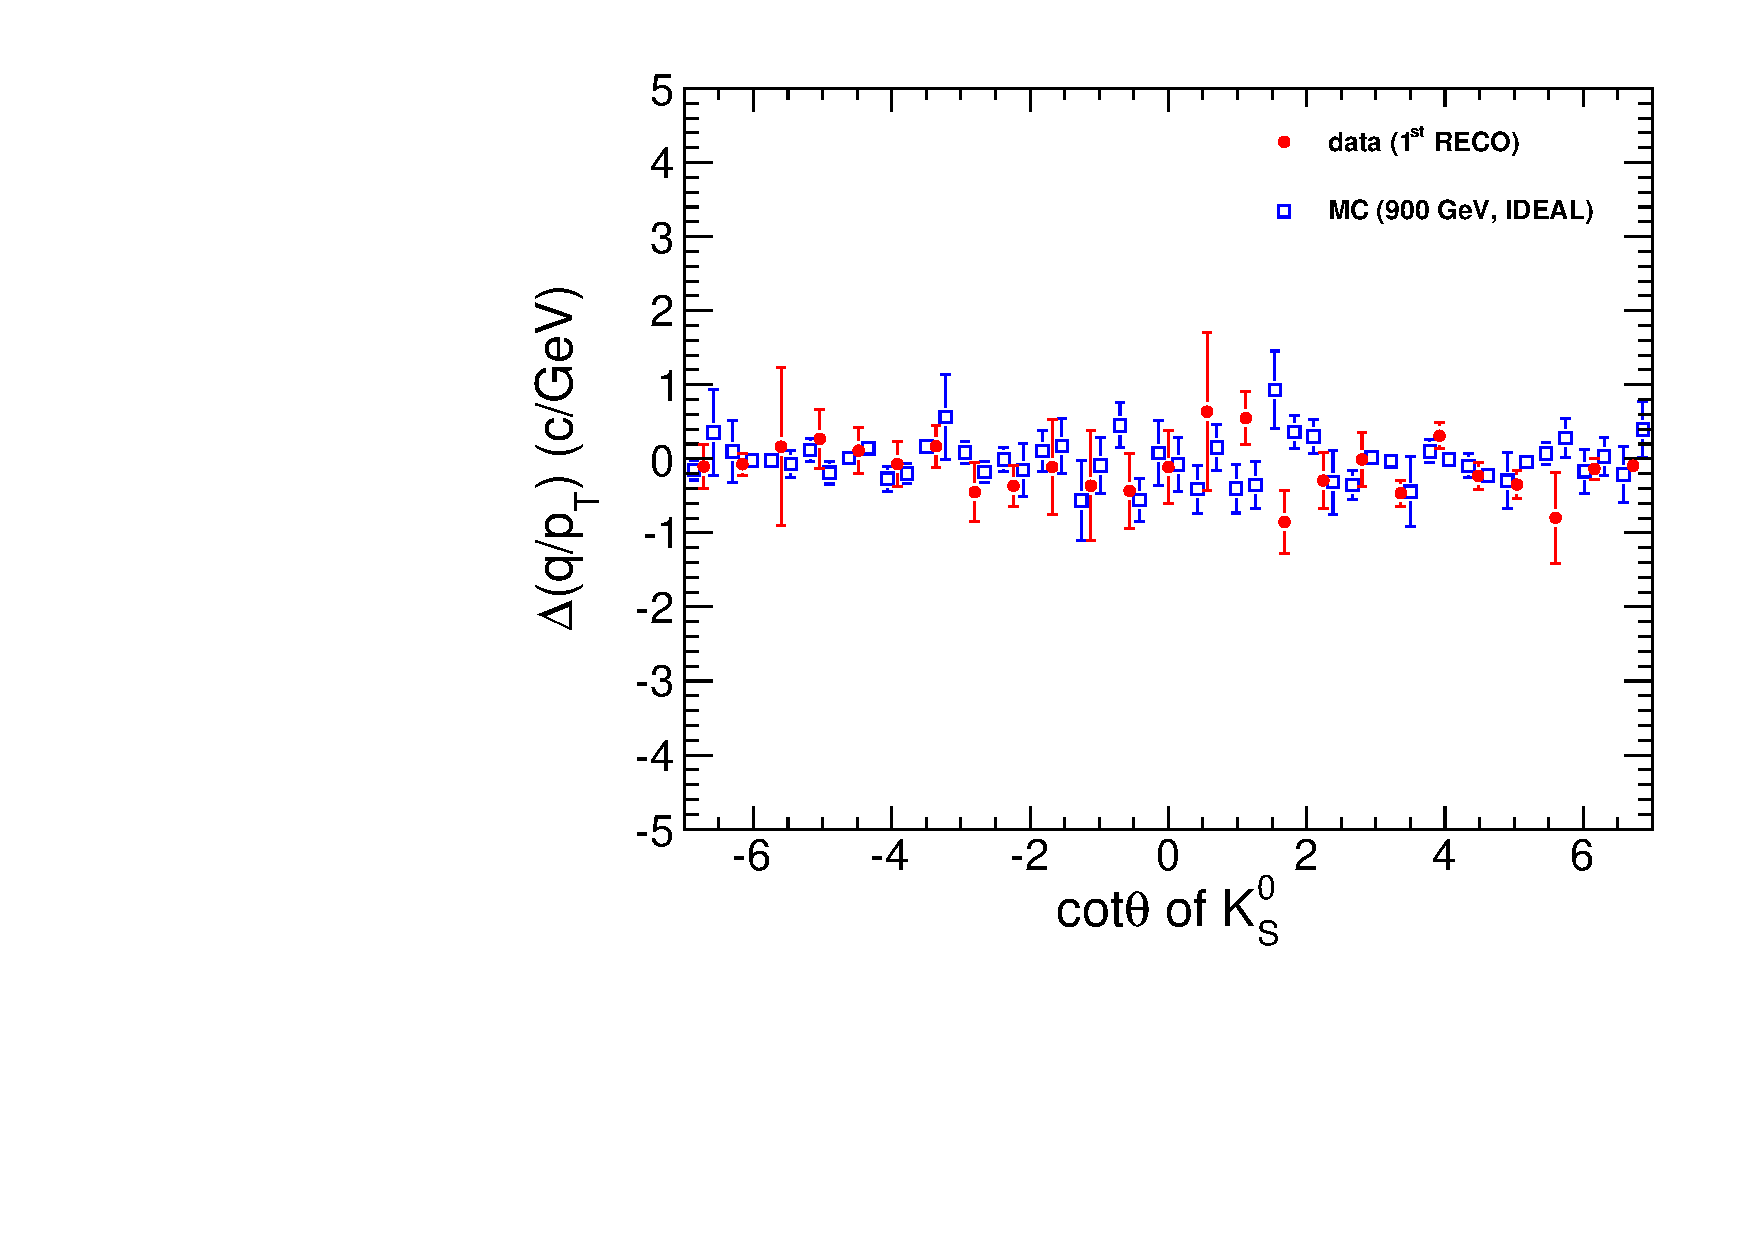
\includegraphics[width=0.32\linewidth]{kaonTracking2_deltaqoverpt_vscottheta.pdf}
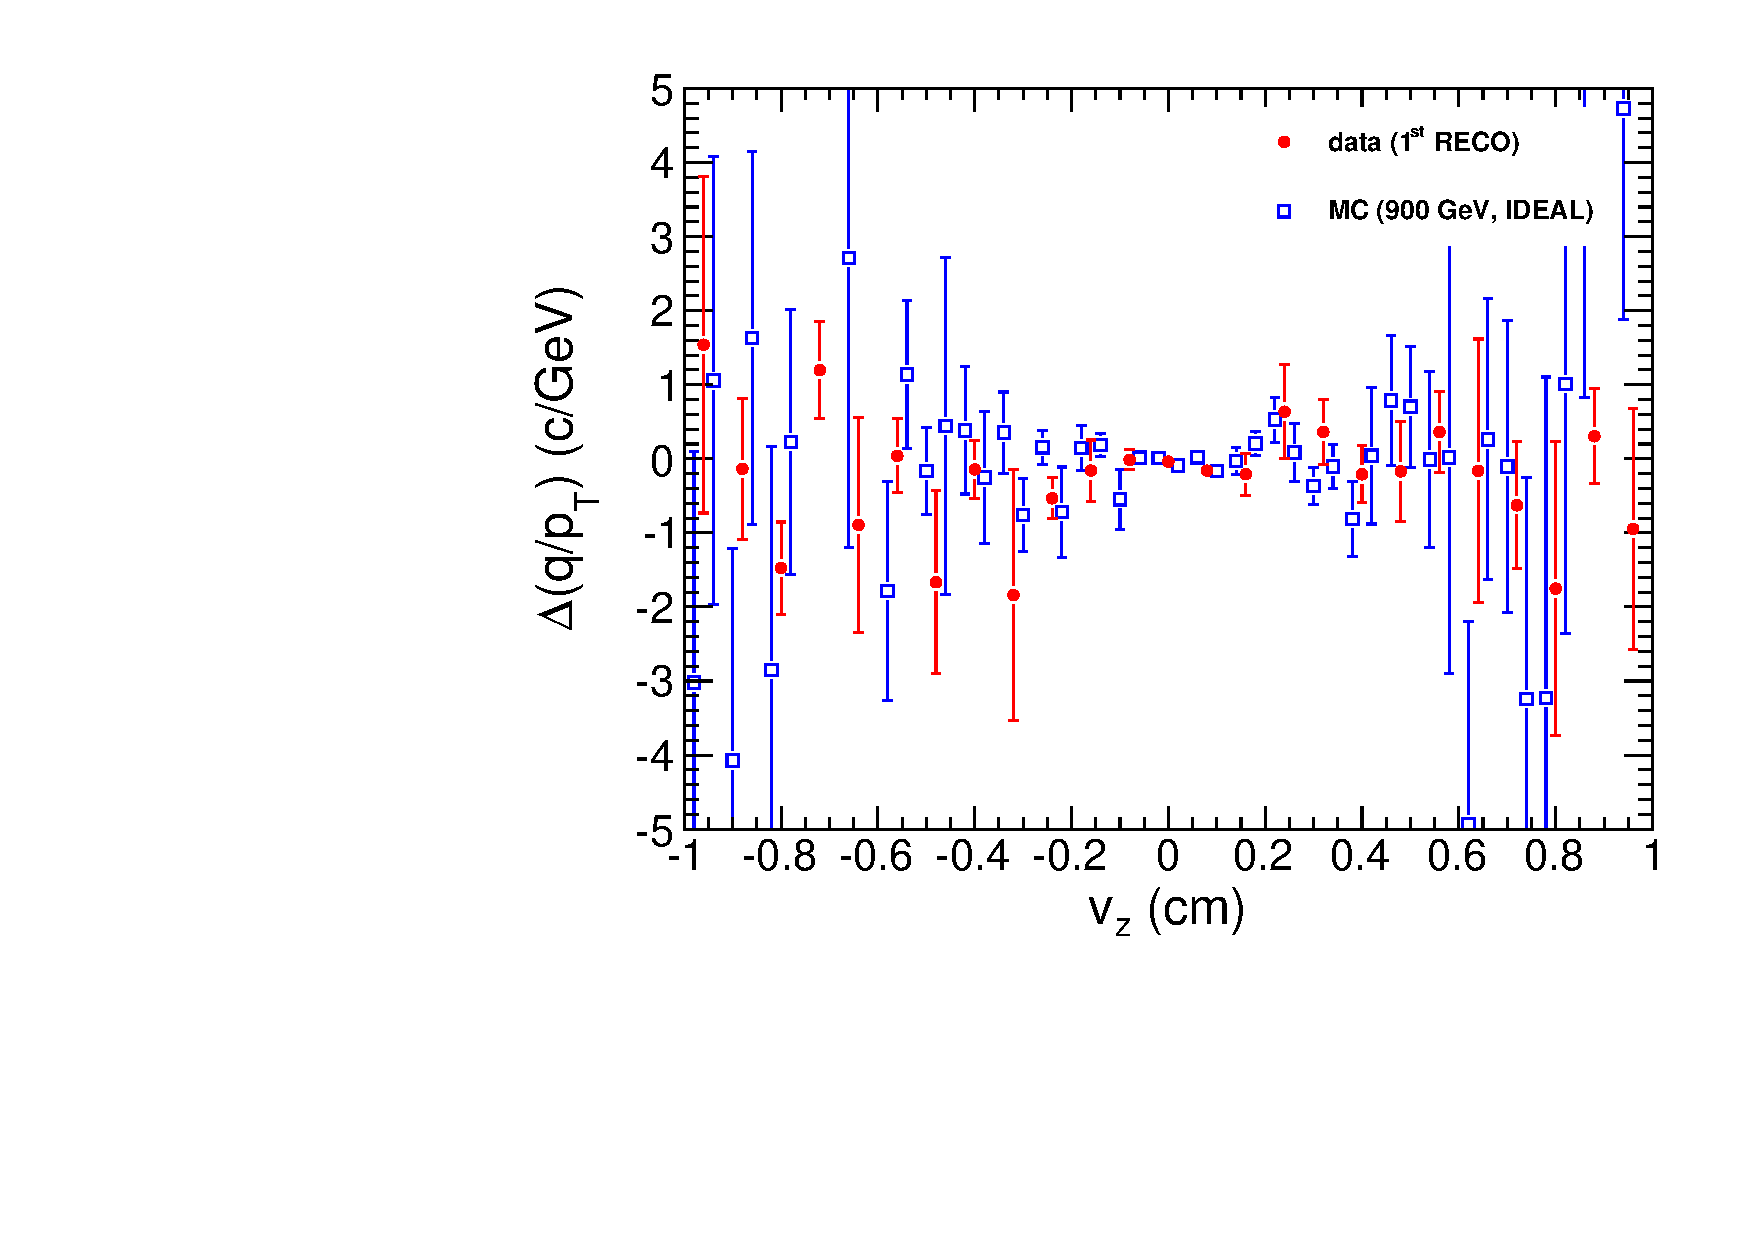
\includegraphics[width=0.32\linewidth]{kaonTracking2_deltaqoverpt_vsvz.pdf}
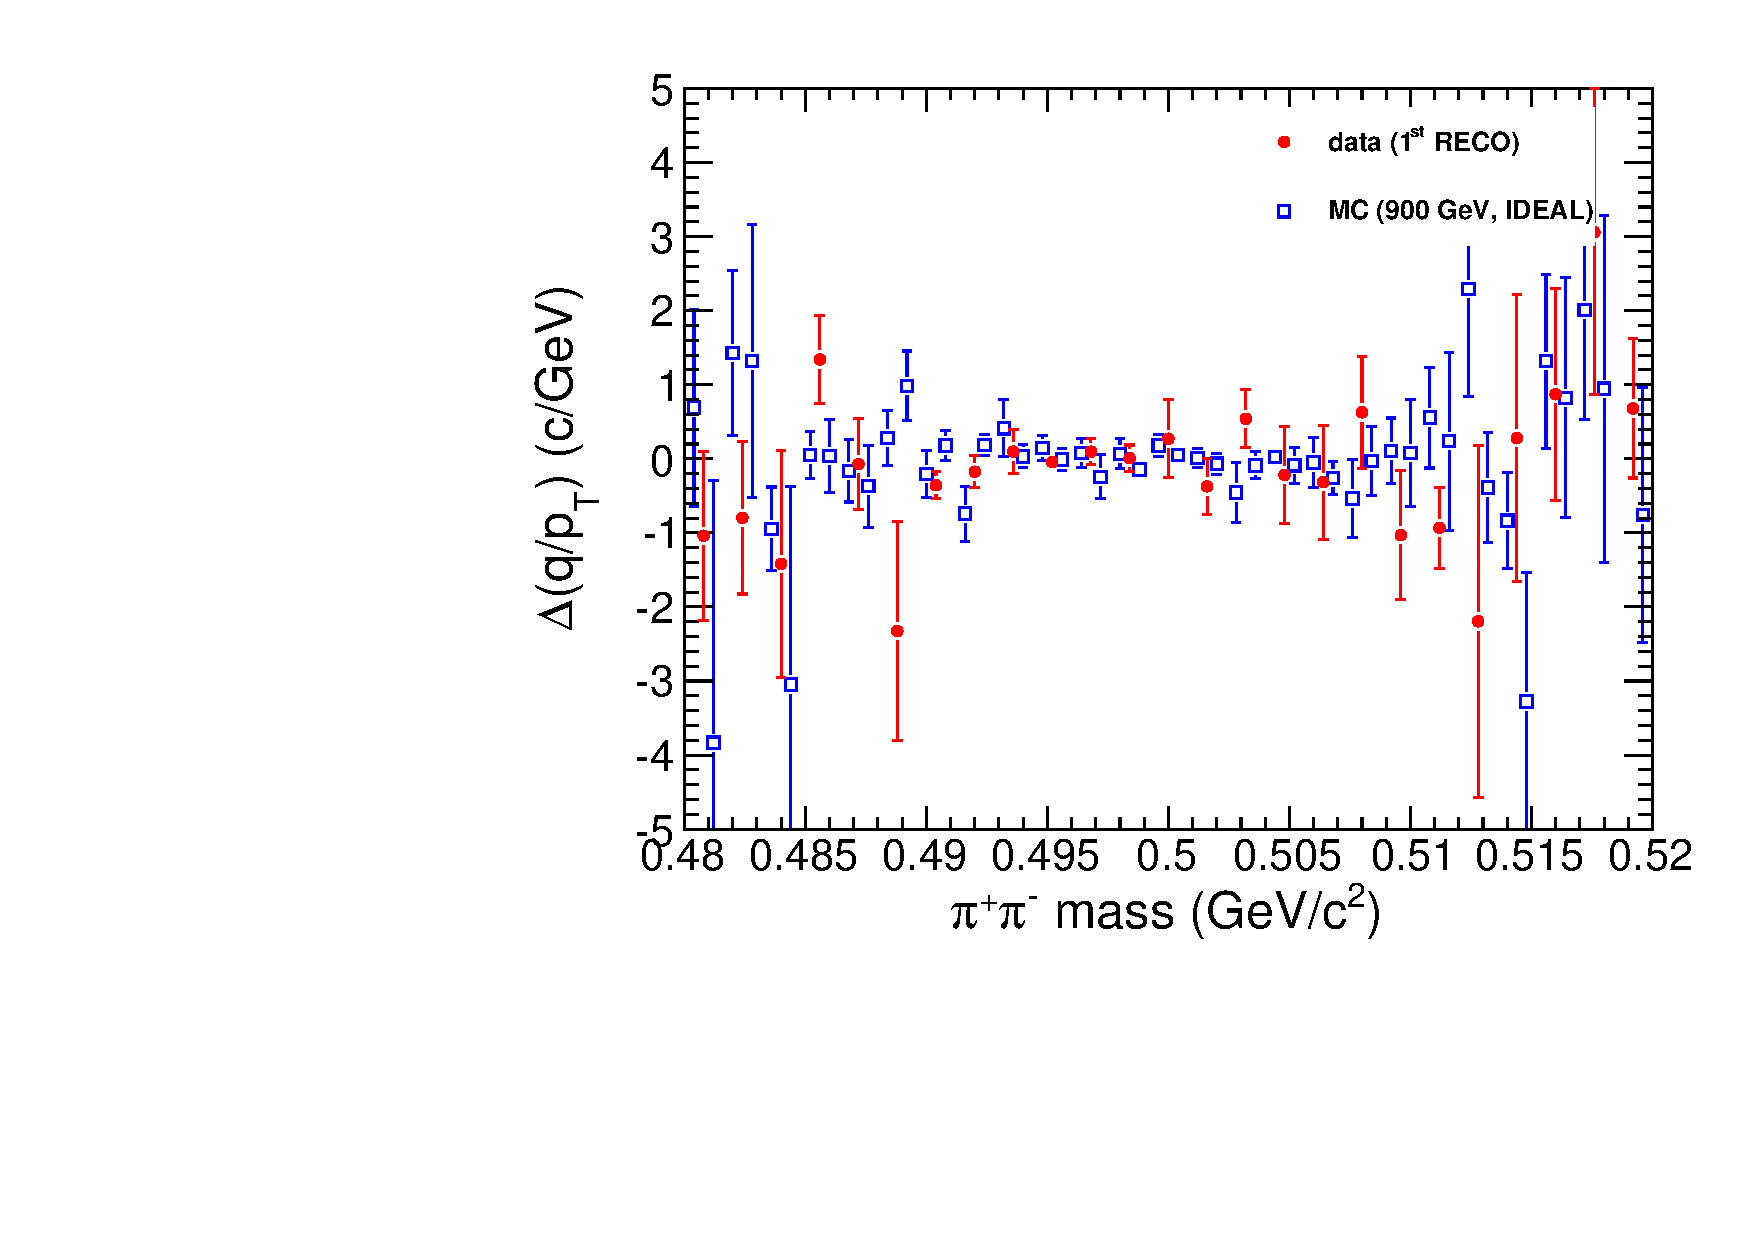
\includegraphics[width=0.32\linewidth]{kaonTracking2_deltaqoverpt_vsmass.pdf}
\end{frame}

%% \section*{First section}
%% \begin{frame}
%% \begin{center}
%% \Huge \textcolor{blue}{First section}
%% \end{center}
%% \end{frame}

\begin{frame}
\frametitle{Conclusions}

\begin{itemize}\setlength{\itemsep}{0.1 cm}
\item ``Muon residuals vs momentum trend'' seems to be related to a
  distortion of the tracker

\item Markus has created a true weak mode of the tracker which
  produces a similar signal in the muon residuals, including the
  curious 100~GeV characteristic scale

\item Muon residuals indicate a high-low bias difference of $\Delta
  \kappa(\mbox{high}) - \Delta \kappa(\mbox{low})$ = $0.000\,5
  \sin\phi$~GeV$^{-1}$

\item Cosmic spectrum endpoint excludes a $\Delta \kappa(\mbox{high})$
  of $0.000\,5$~GeV$^{-1}$, more like $0.000\,05$~GeV$^{-1}$

\item $K_S \to \pi^+\pi^-$ direction constraint is weak, $\Delta
  \kappa(\mbox{low}) = -0.000\,3 \pm 0.002\,4$~GeV$^{-1}$
\begin{itemize}
\item would improve with statistics

\item perhaps $K_S$ can help to constrain alignment procedure?
\end{itemize}

\item Just as importantly: uncertainties on $\Delta \kappa(p_T, \phi, \theta)$ as a
  deliverable to physics analyses?
\end{itemize}

\label{numpages}
\end{frame}

\end{document}
